%% \chapter[htoc-titlei][hhead-titlei]{htitlei}
%% -----------------------------------------------------------------------------
\chapter[B-L stop search][B-L stop search]{B-L stop search}
\label{ch:bl_stop}

{\color{red}A lot of this chapter is just going to be lifted from the CONF note
  and then expanded upon. The section headings are mostly the same}

%% -----------------------------------------------------------------------------
\section{Object selection}
\label{sec:object_selection}

Events are required to have at least two leptons with opposite charge, and two
$b$-tagged jets.
The object selection is performed in multiple steps. First, lepton and jet
objects are reconstructed using detector signatures as described in
Sections~\ref{sec:elctrons},~\ref{sec:muons},~and~\ref{sec:jets}.
Baseline requirements are applied to remove poorly reconstructed objects.
Also, all baseline objects are required to have $\pt \geq 40 \GeV$ since the
stop signatures of interest tend to produce high momentum decay products.

Baseline electrons must satisfy the \texttt{Medium++} identification
requirement and have $|\eta| \leq 2.47$.
In order to ensure the electron is prompt, requirements of 
$d_0/\sigma(d_0) \leq 3$ and $z_0\,sin(\theta) \leq 0.4$ mm was placed on the
impact parameter. The baseline electron requirements are outlined in
Table~\ref{tab:baseline_el_def}.

\begin{table}[ht]
\caption{Baseline electron requirements.}
\label{tab:baseline_el_def}
\centering{
  \begin{tabular}{cc}
  \toprule
    Quality            & \texttt{Medium++} \\
    $p_T$              & $\geq 40$ GeV      \\
    $|\eta|$           & $\leq 2.47$        \\
    $d_0/\sigma(d_0)$  & $\leq 3$           \\
    $z_0\,sin(\theta)$ & $\leq 0.4$ mm      \\
    \bottomrule
    \end{tabular}
}
\end{table}

\begin{table}[ht]
    \caption{Baseline muon requirements.}
    \label{tab:baseline_mu_def}
  \centering{
    \begin{tabular}{cc}
      \toprule
      Quality              & \texttt{Loose} \\
      $p_T$                & $\ge 40$ GeV   \\
      $|\eta|$             & $\le 2.5$      \\
      Number B layer hits  & $\ge 1$        \\
      Number Pixel hits    & $\ge 1$        \\
      Number SCT hits      & $\ge 5$        \\
      Number Silicon holes & $\le 2$        \\
      TRT hits             & See text       \\
      $d_0/\sigma(d_0)$    & $\le 3$        \\
      $z_0\,\sin(\theta)$  & $\le 1$ mm     \\
      \bottomrule
    \end{tabular}
  }
\end{table}

\begin{table}[ht]
    \caption{Baseline jet requirements.}
    \label{tab:baseline_jet_def}
  \centering{
    \begin{tabular}{cc}
      \toprule
      $p_T$    & $\ge 40$ GeV \\
      $|\eta|$ & $\le 4.9$    \\
      \bottomrule
    \end{tabular}
  }
\end{table}

\begin{enumerate}
  \item $\Delta R(e,e) \le 0.05$: If two baseline electrons fall
    within a cone of $\Delta R(e,e) \le 0.05$, the electron with the
    lower transverse energy ($E_T$) is removed from the event.
  \item $\Delta R(e,\mathrm{jet}) \le 0.20$: If an electron and a jet
    are within a cone of $\Delta R(e,\mathrm{jet}) \le 0.20$, it is
    assumed that the electron is also reconstructed as a jet, and the
    jet is removed from the event.
  \item $\Delta R(e,\mathrm{jet}) \le 0.40$: If an electron an a jet
    are within a cone of $\Delta R(e,\mathrm{jet}) \le 0.40$ after the
    previous step, the reconstructed electron is assumed to be a
    constituent of the jet, and is removed from the event.
  \item $\Delta R(\mu,\mathrm{jet}) \le 0.40$: If a muon and a jet are
    within a cone of $\Delta R(\mu,\mathrm{jet}) \le 0.40$, the muon
    is assumed to be a constituent of the jet, and is removed from the
    event.
  \item $\Delta R(e,\mu) \le 0.01$: If an electron and a muon are
    within $\Delta R(e,\mu) \le 0.01$, both are removed from the
    event.
  \item $\Delta R(\mu,\mu) \le 0.05$: If two muons are within $\Delta
    R(\mu,\mu) \le 0.05$, both are removed from the event.
\end{enumerate}

If more than two signal leptons or two $b$-tagged jets are found, the event is
kept, but only the two signal leptons and two $b$-tagged jets with the highest
\pt\ are selected.

%% - - - - - - - - - - - - - - - - - - - - - - - - - - - - - - - - - - - - - - -
% Define some colors for this section to make changing colors easier
\colorlet{pairing_l_0}{green!50!white}
\colorlet{pairing_l_1}{green!20!white}
\colorlet{pairing_b_0}{red!50!white}
\colorlet{pairing_b_1}{red!20!white}
%
\begin{center}
  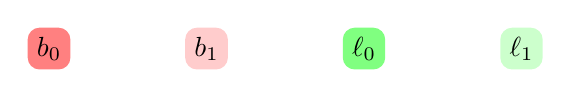
\begin{tikzpicture}
    \node[rectangle, rounded corners=1ex, fill=pairing_b_0, text=black] (b0) at (-3,0) {$b_0$};
    \node[rectangle, rounded corners=1ex, fill=pairing_b_1, text=black] (b1) at (-1,0) {$b_1$};
    \node[rectangle, rounded corners=1ex, fill=pairing_l_0, text=black] (l0) at (+1,0) {$\ell_0$};
    \node[rectangle, rounded corners=1ex, fill=pairing_l_1, text=black] (l1) at (+3,0) {$\ell_1$};
  \end{tikzpicture}
\end{center}
%
There are two possible choices of pairings for these four objects.
%
\begin{center}
  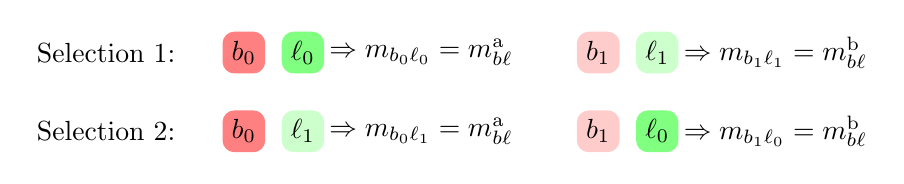
\begin{tikzpicture}
    \node[rectangle, text=black] (sel1) at (-5.0,+0.5) {Selection 1:};
    \node[rectangle, text=black] (sel2) at (-5.0,-0.5) {Selection 2:};

    \node[rectangle, rounded corners=1ex, fill=pairing_b_0, text=black] (b1) at (-3.25,+0.5) {$b_0$};
    \node[rectangle, rounded corners=1ex, fill=pairing_l_0, text=black] (l0) at (-2.50,+0.5) {$\ell_0$};
    \node[rectangle, rounded corners=1ex, fill=pairing_b_1, text=black] (b1) at (+1.25,+0.5) {$b_1$};
    \node[rectangle, rounded corners=1ex, fill=pairing_l_1, text=black] (l1) at (+2.00,+0.5) {$\ell_1$};
    \node[rectangle, text=black] (m00) at (-1.0,+0.5) {$\Rightarrow m_{b_0\ell_0} = m_{b\ell}^\mathrm{a}$};
    \node[rectangle, text=black] (m11) at (+3.5,+0.5) {$\Rightarrow m_{b_1\ell_1} = m_{b\ell}^\mathrm{b}$};

    \node[rectangle, rounded corners=1ex, fill=pairing_b_0, text=black] (b0) at (-3.25,-0.5) {$b_0$};
    \node[rectangle, rounded corners=1ex, fill=pairing_l_1, text=black] (l1) at (-2.50,-0.5) {$\ell_1$};
    \node[rectangle, rounded corners=1ex, fill=pairing_b_1, text=black] (b1) at (+1.25,-0.5) {$b_1$};
    \node[rectangle, rounded corners=1ex, fill=pairing_l_0, text=black] (l0) at (+2.00,-0.5) {$\ell_0$};
    \node[rectangle, text=black] (m01) at (-1.0,-0.5) {$\Rightarrow m_{b_0\ell_1} = m_{b\ell}^\mathrm{a} $};
    \node[rectangle, text=black] (m10) at (+3.5,-0.5) {$\Rightarrow m_{b_1\ell_0} = m_{b\ell}^\mathrm{b} $};
  \end{tikzpicture}
\end{center}
%% - - - - - - - - - - - - - - - - - - - - - - - - - - - - - - - - - - - - - - -

\section{Trigger selection}
\label{sec:trigger_selection}

{\color{red} Expand on this a lot}

Single-electron and single-muon triggers are used to select events. 
Di-electron and di-muon events are required to pass a single-electron and
single-muon trigger respectively, while electron-muon events are selected if
either or both of the single-lepton triggers are passed.
At least one of the reconstructed leptons is required to be
within $\Delta R \leq 0.15$ of the detector signature found by the trigger.
This trigger requirement is highly efficient for signal events; between 93\%
and 98\% of events depending on the flavor channel.

\begin{table}[ht]
    \caption{Requirements for the triggers used in this analysis.  }
    \label{tab:trigger_defs}
  \centering{
    \begin{tabular}{c|cc}
      \toprule
      Trigger & $p_\mathrm{T}$ threshold & Other requirements \\
      \midrule
      \multirow{2}{*}{\texttt{EF\_e24vhi\_medium1}}
      & \multirow{2}{*}{$p_\mathrm{T}^{e} \ge 24$ GeV}
      & hadronic core isolation $\le 1$ GeV \\
      & & $p_\mathrm{T}^\mathrm{cone20}/p\mathrm{T} < 0.1$ \\
      \texttt{EF\_e60\_medium1} & $p_\mathrm{T}^{e} \ge 60$ GeV & -- \\
      \texttt{EF\_mu24i\_tight}
      & $p_\mathrm{T}^{e} \ge 24$ GeV
      & $p_\mathrm{T}^\mathrm{cone20}/p\mathrm{T} < 0.12$ \\
      \texttt{EF\_mu36\_tight}  & $p_\mathrm{T}^{e} \ge 36$ GeV & -- \\
      \bottomrule
    \end{tabular}
  }
\end{table}

\begin{figure}[ht]
  \centering
  \subbottom[\texttt{EF\_e24vhi\_medium1}]{
    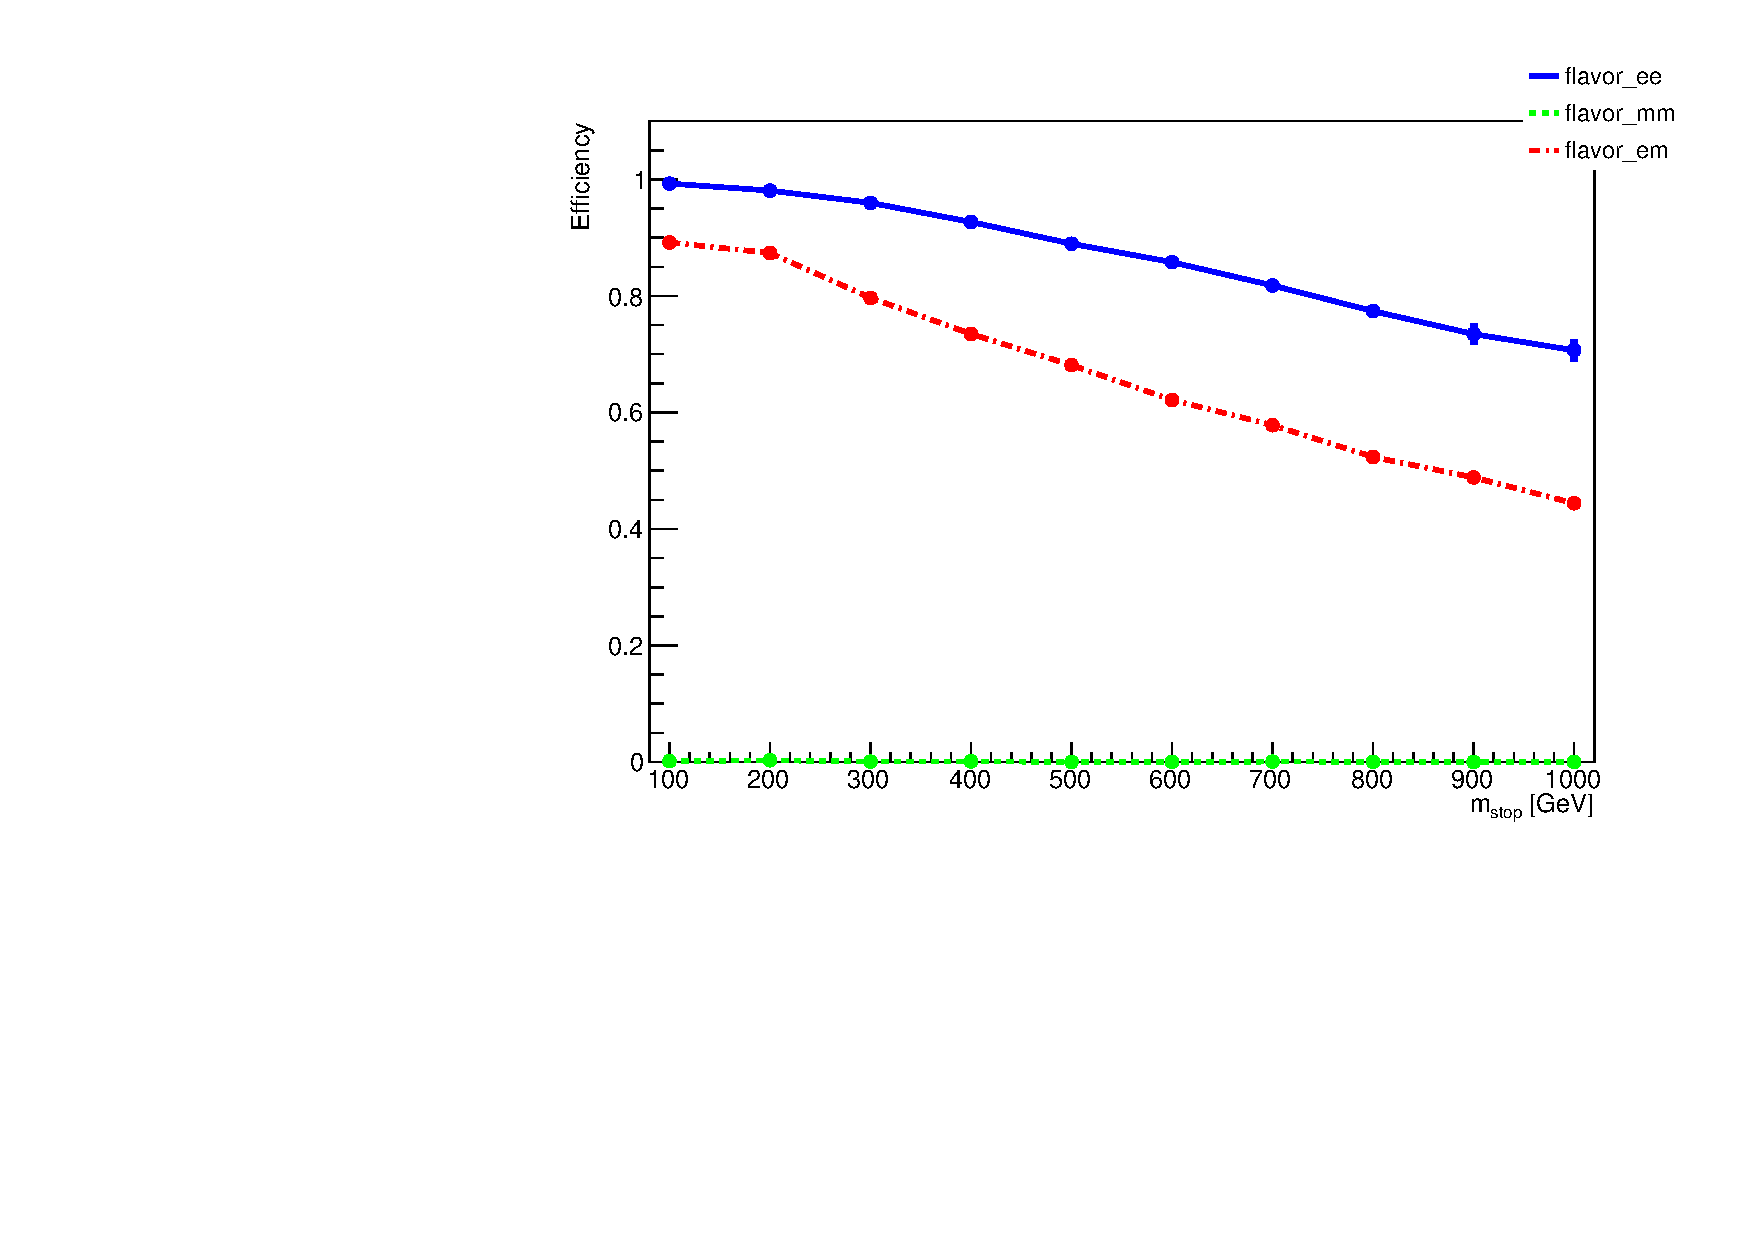
\includegraphics[width=0.45\textwidth]{figs/trigger/EF_e24vhi_medium1.pdf}
  }
  \subbottom[\texttt{EF\_e60\_medium1}]{
    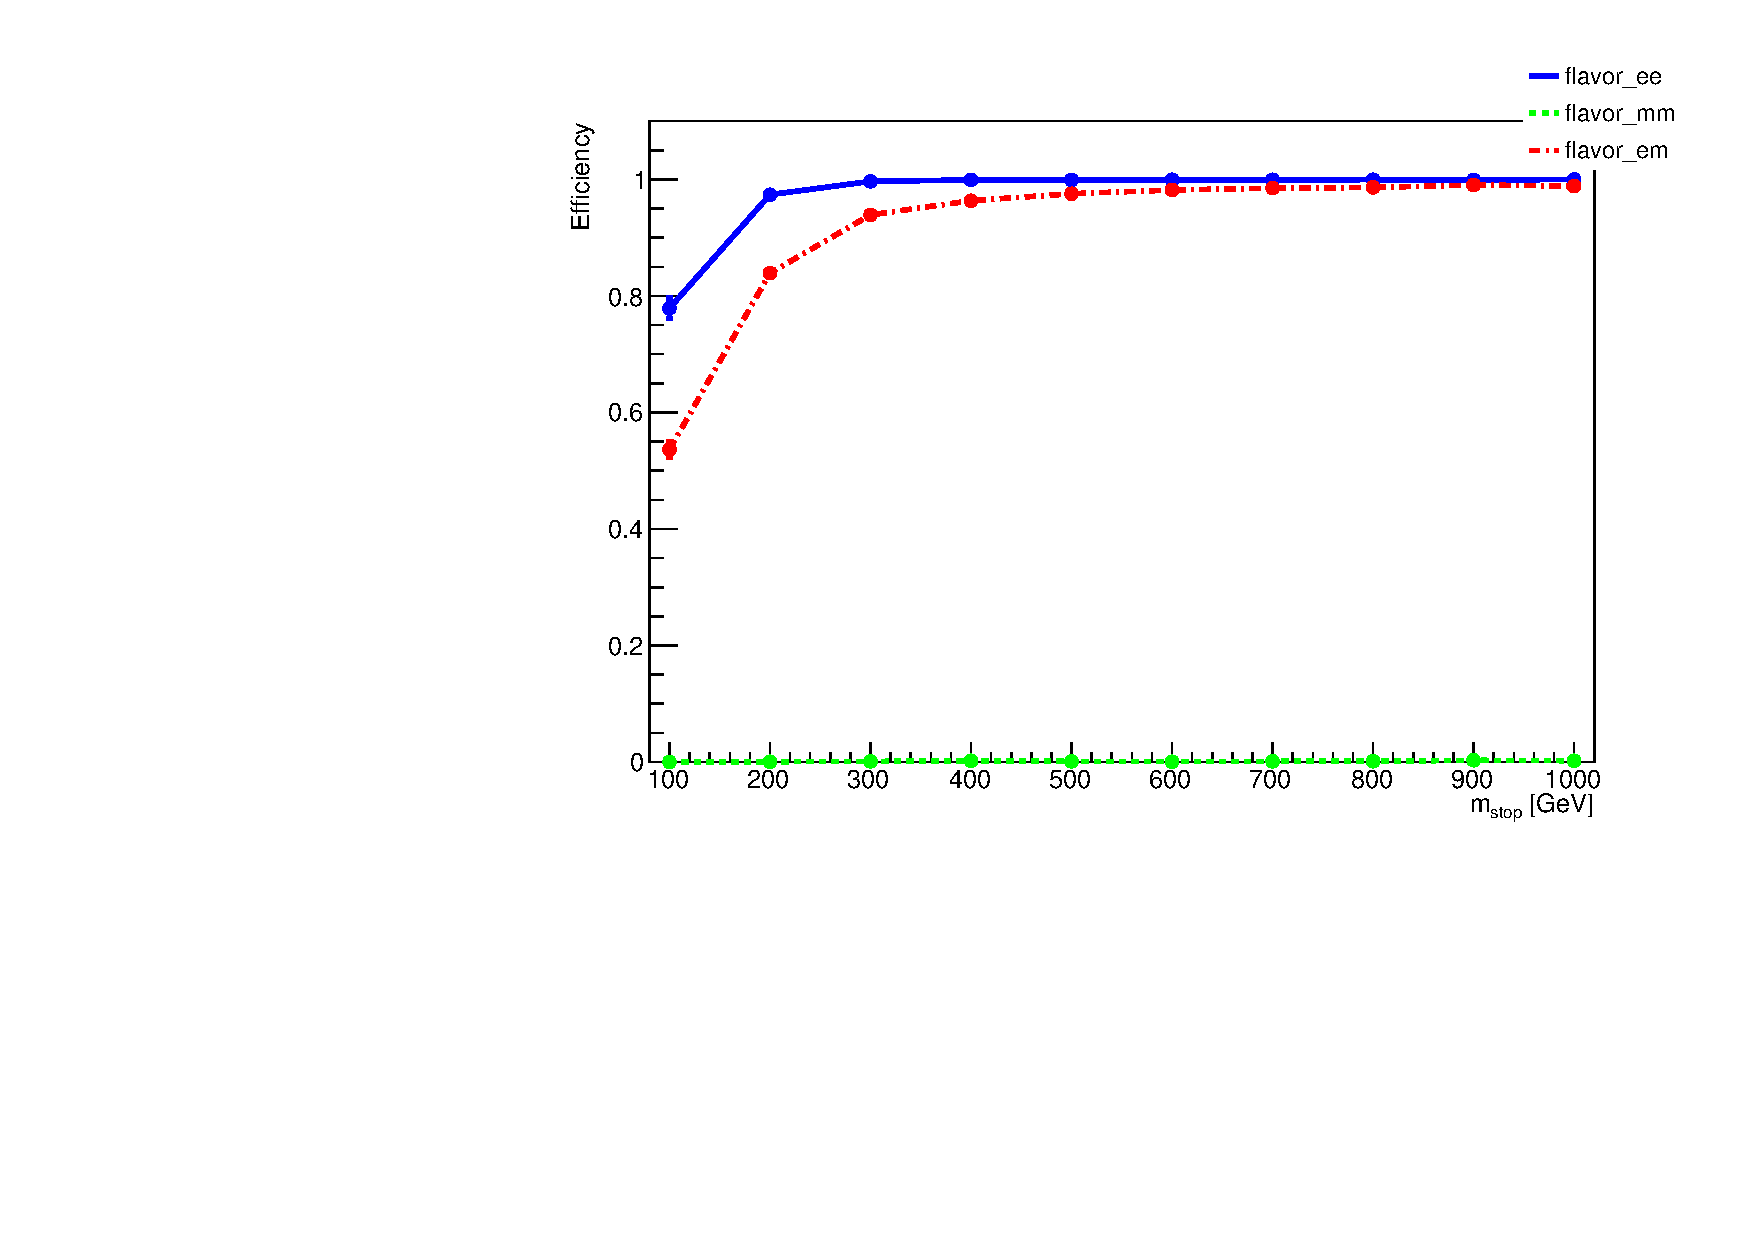
\includegraphics[width=0.45\textwidth]{figs/trigger/EF_e60_medium1.pdf}
  }
  \subbottom[\texttt{EF\_mu24i\_tight trigger}]{
    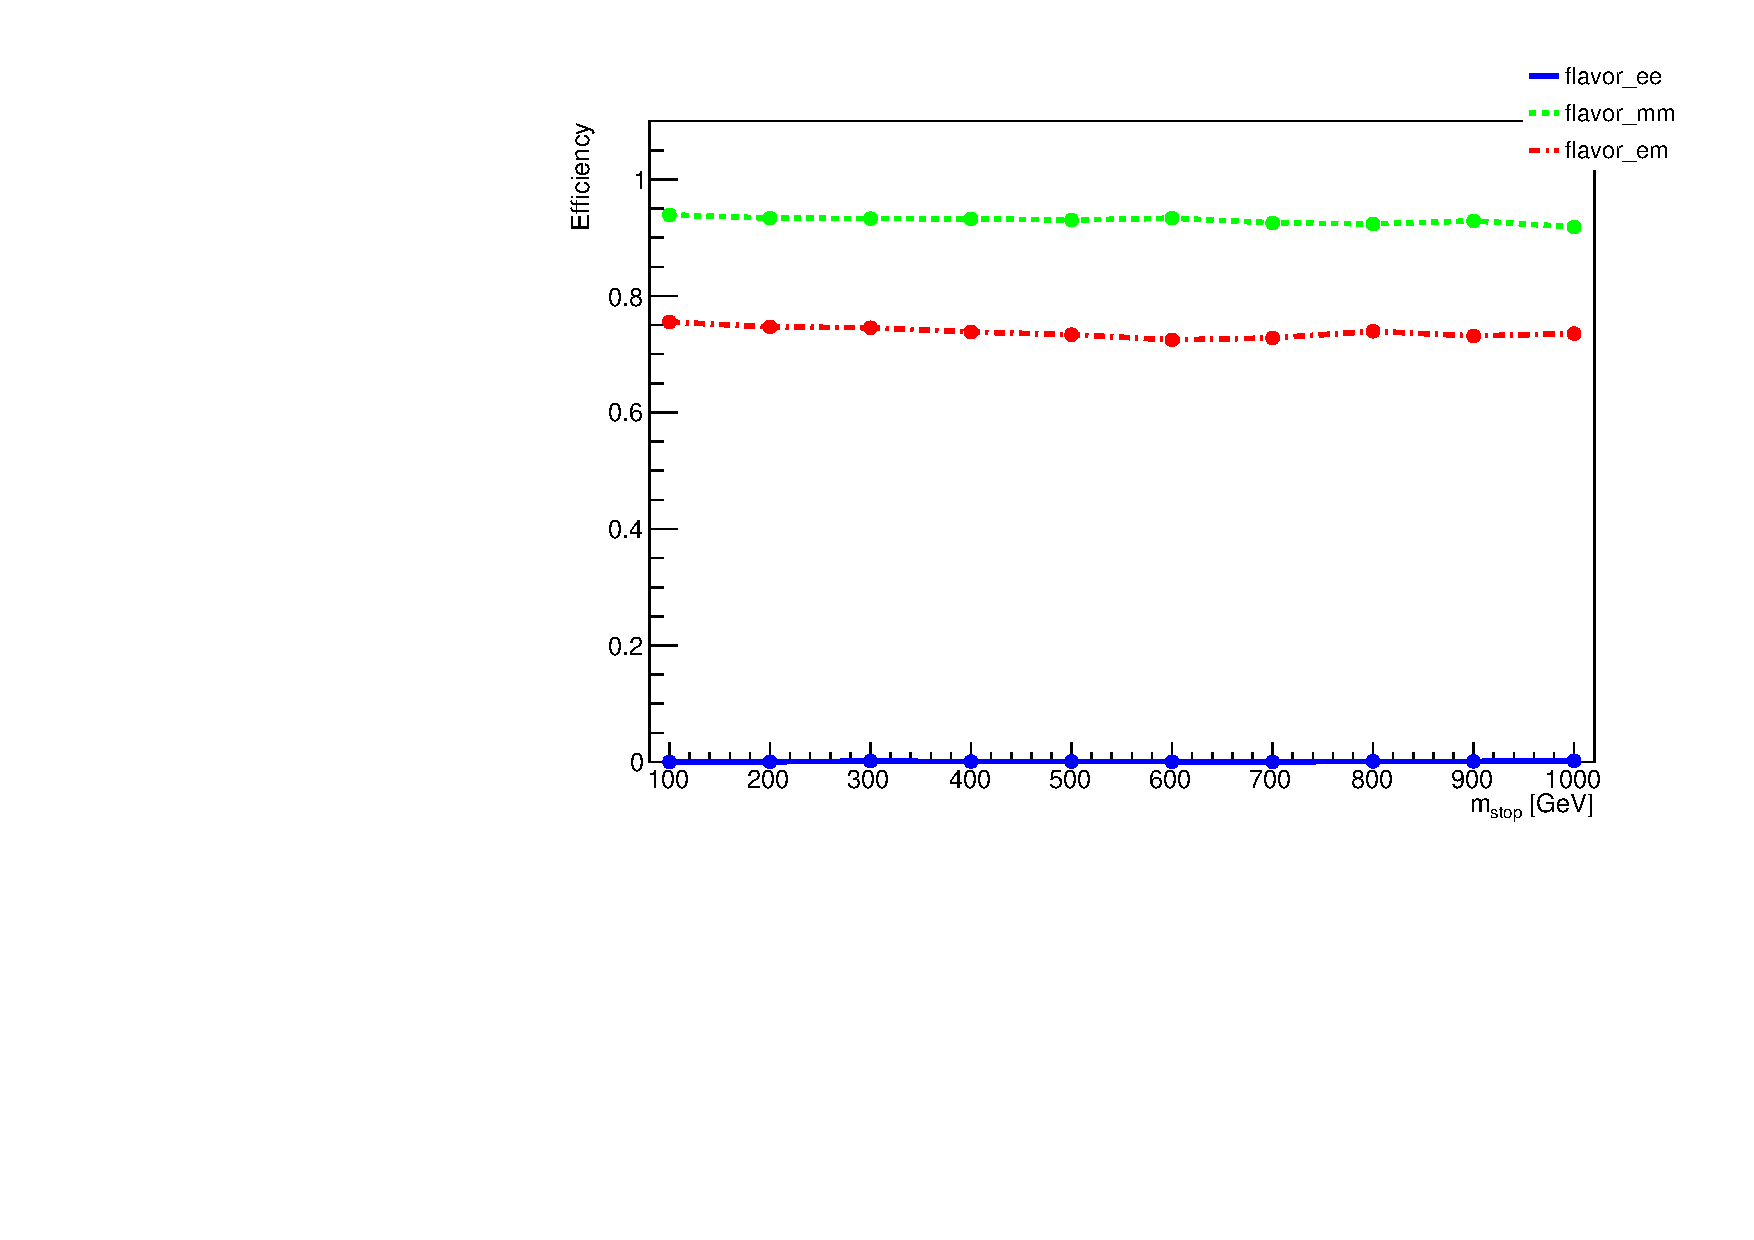
\includegraphics[width=0.45\textwidth]{figs/trigger/EF_mu24i_tight.pdf}
  }
  \subbottom[\texttt{EF\_mu36\_tight}]{
    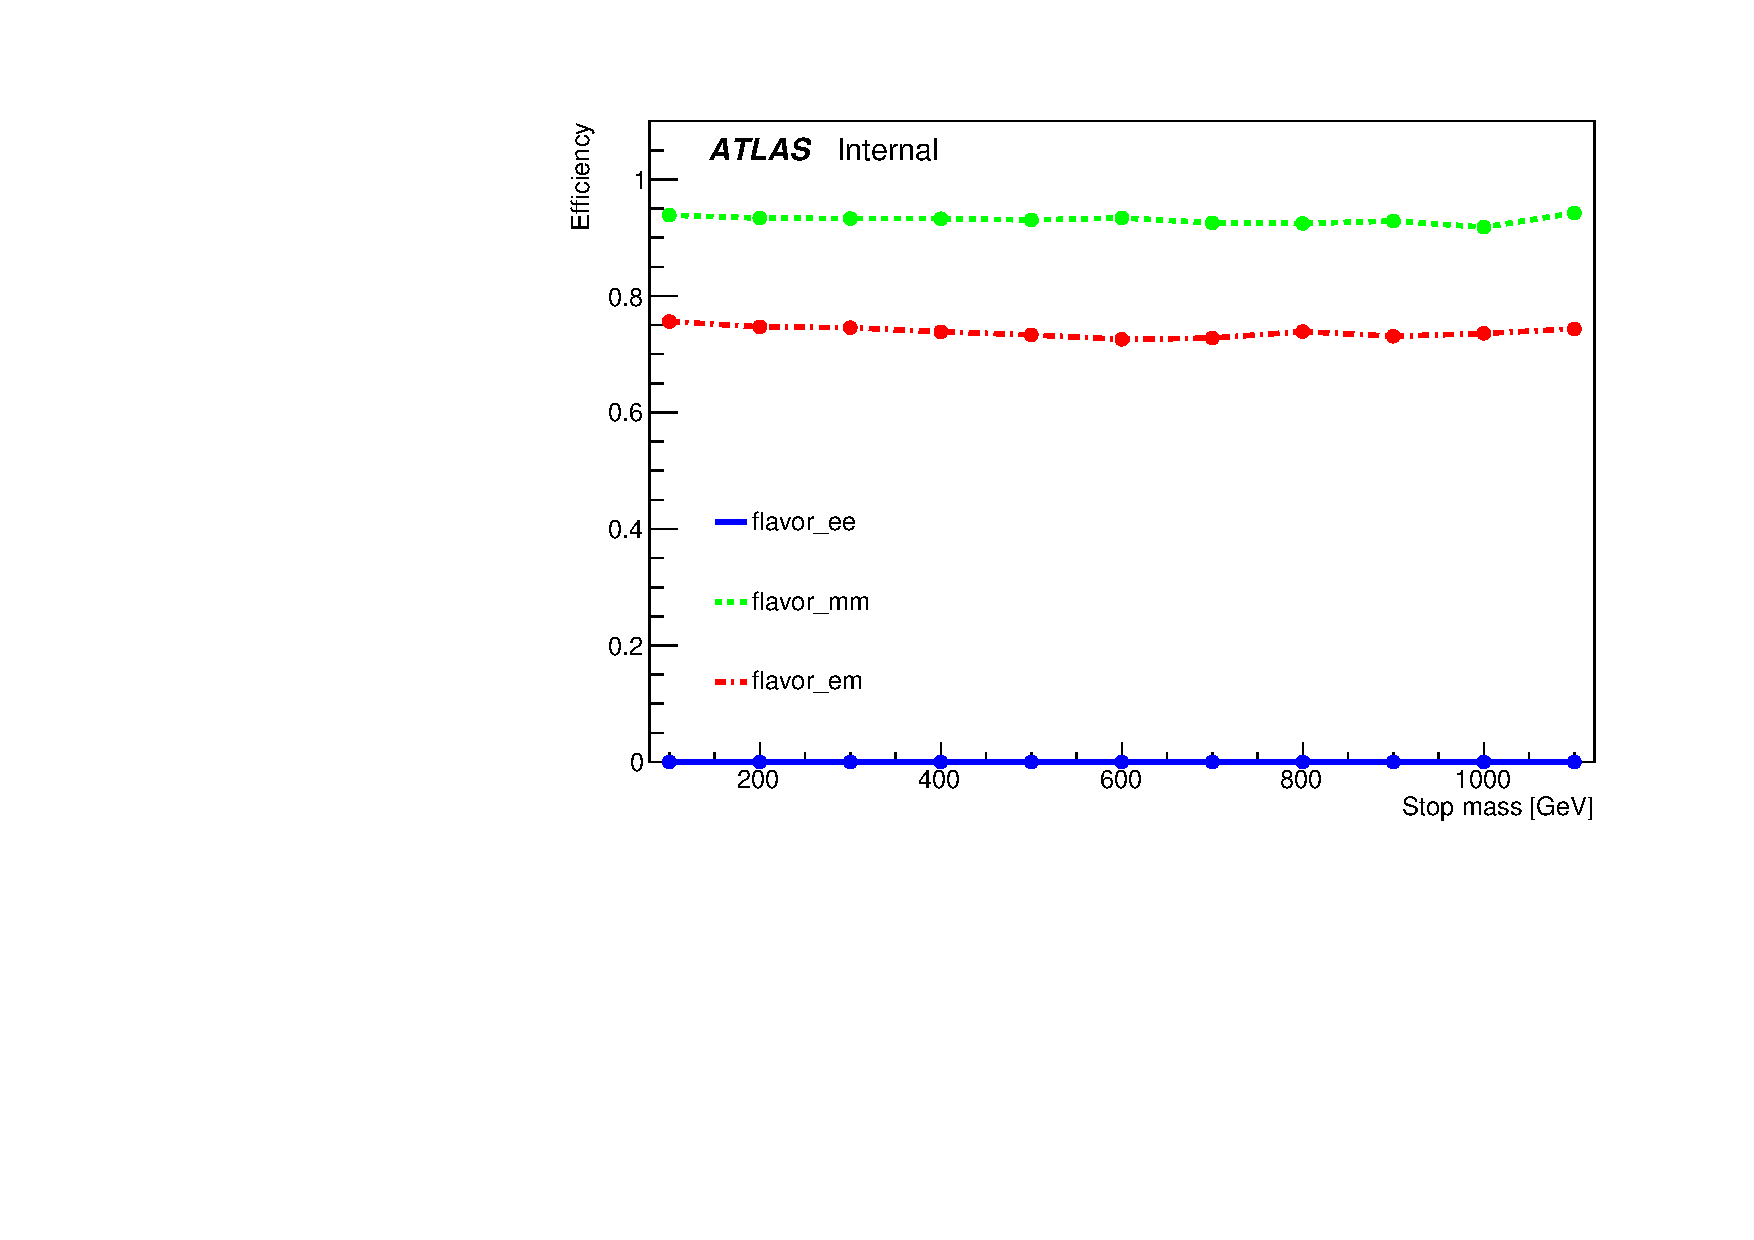
\includegraphics[width=0.45\textwidth]{figs/trigger/EF_mu36_tight.pdf}
  }
  \caption{Efficiency of passing each trigger broken down by flavor channel.}
\end{figure}

\begin{figure}[ht]
  \centering
  \subbottom[\texttt{EF\_e24vhi\_medium1}]{
    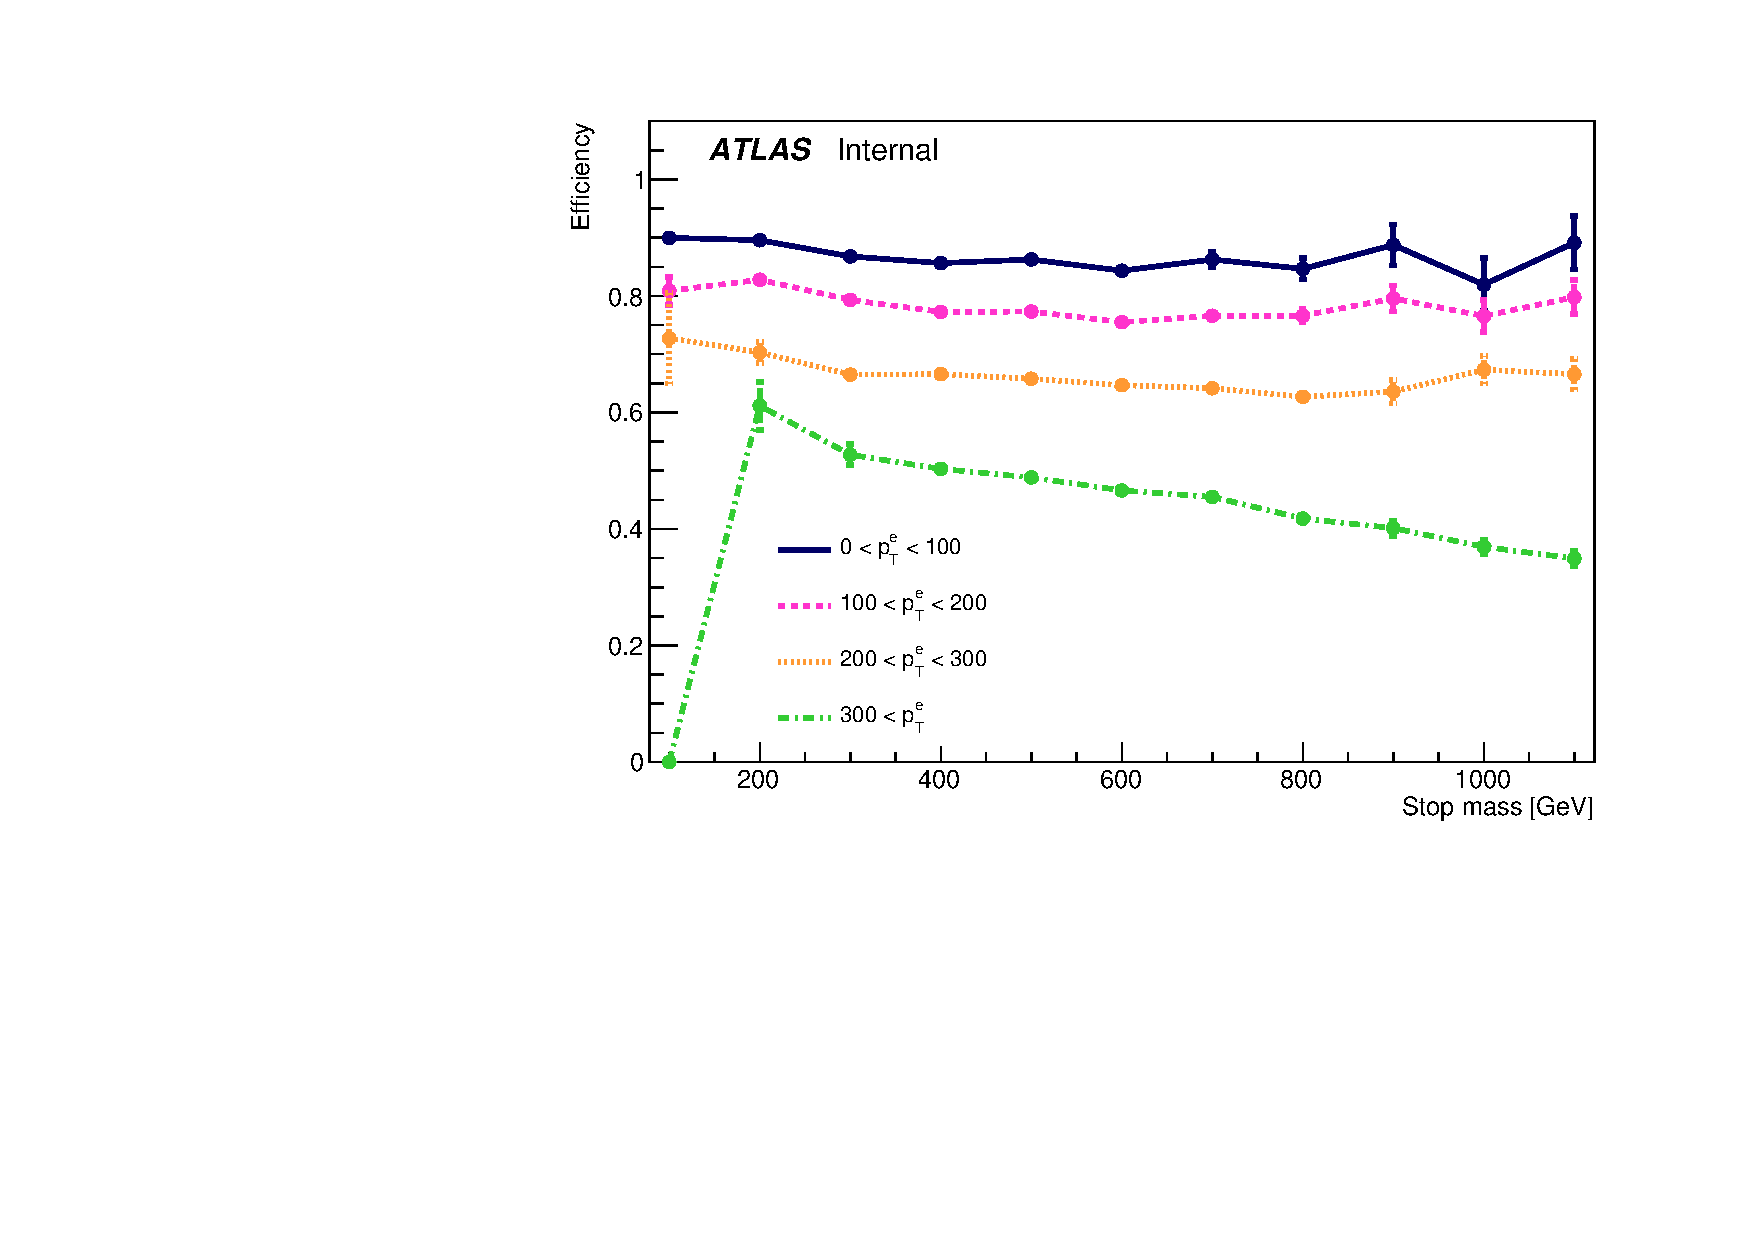
\includegraphics[width=0.45\textwidth]{figs/trigger/EF_e24vhi_medium1__el_pt.pdf}
  }
  \subbottom[\texttt{EF\_e60\_medium1}]{
    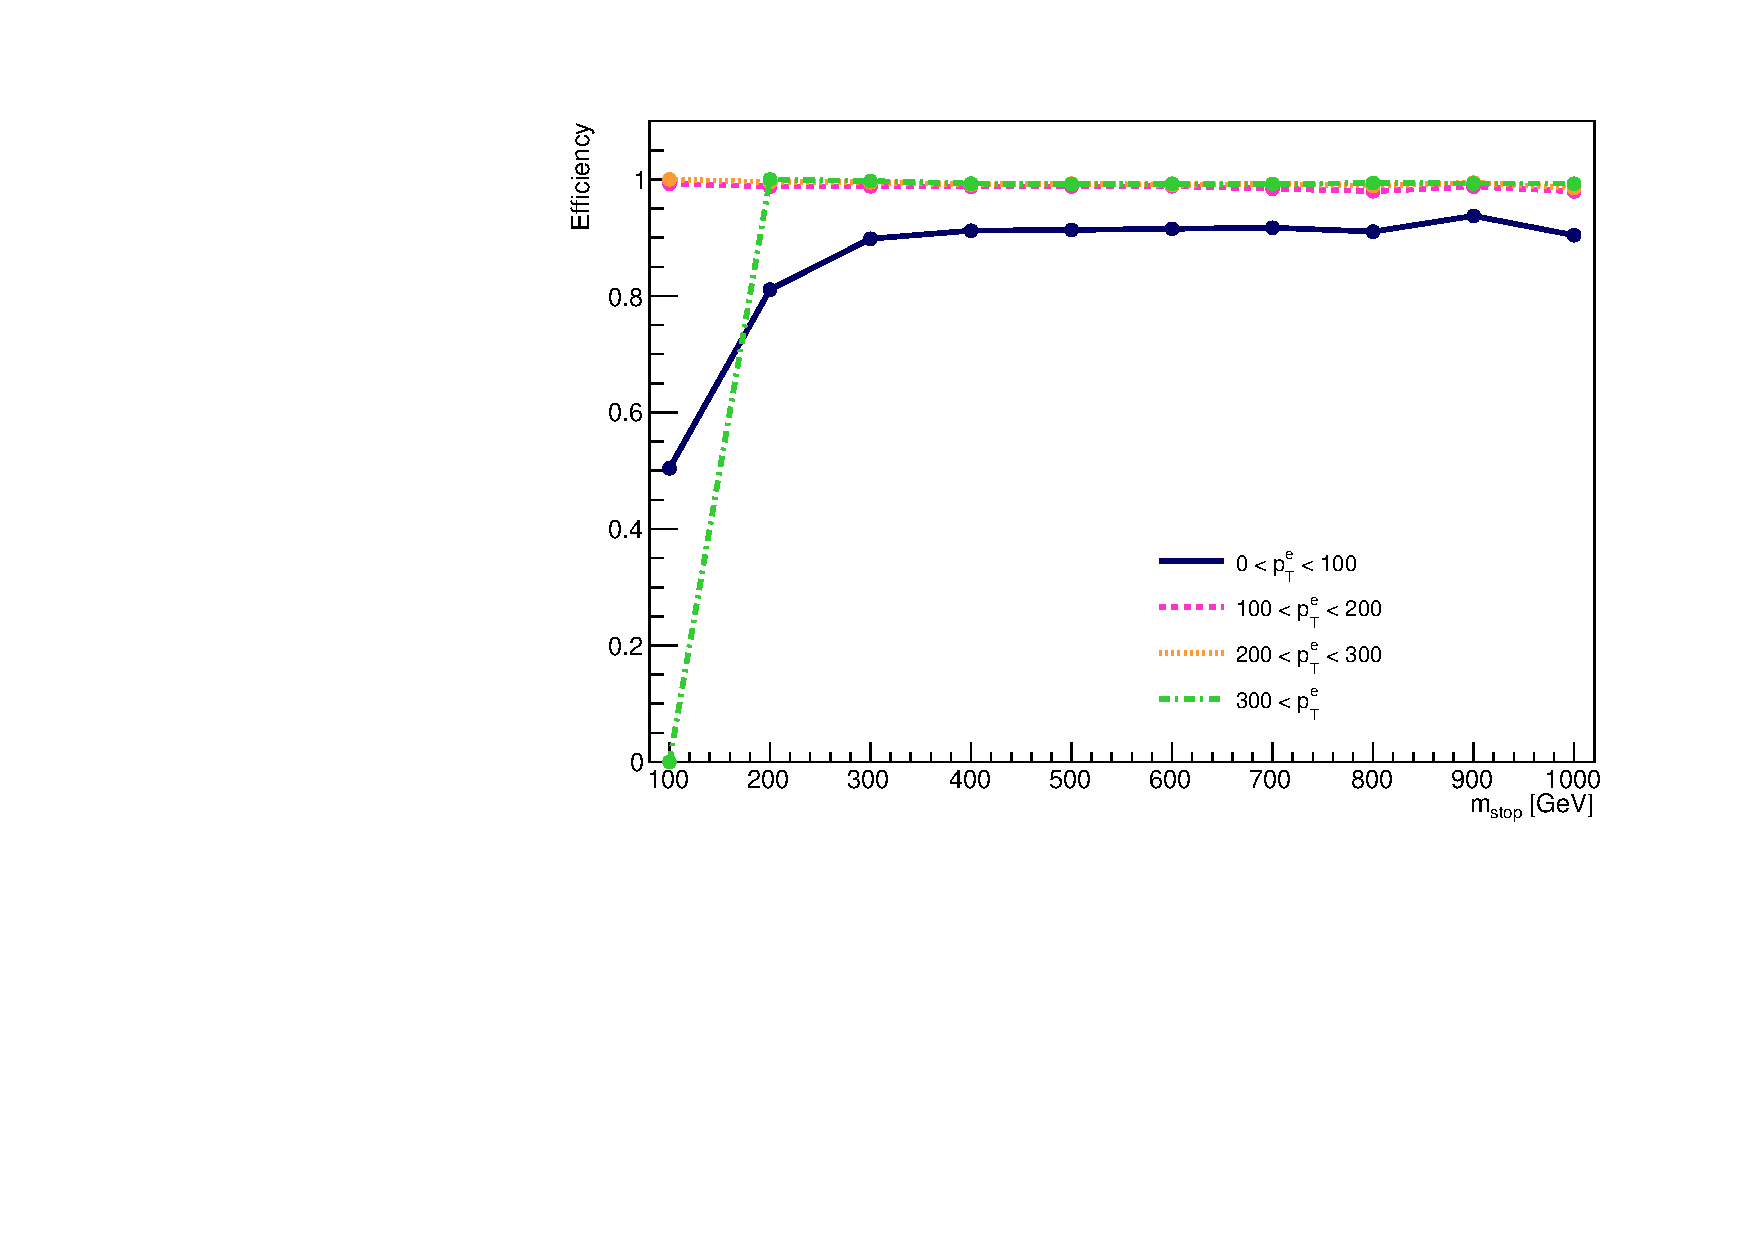
\includegraphics[width=0.45\textwidth]{figs/trigger/EF_e60_medium1__el_pt.pdf}
  }
  \caption{Efficiency of passing the single electron triggers for several
    ranges of electron transverse momentum. Only flavor\_em events are shown.
  }
\end{figure}

\begin{table}[ht]
  \caption{Trigger selection for each final state. If the event passes any of
    the triggers for the given final state, the event is accepted.
  }
  \label{tab:triggers}
  \centering{
    \begin{tabular}{cc}
      \toprule
      Final state & Trigger \\
      \midrule
      \multirow{2}{*}{$ee$bb}     &  \texttt{EF\_e24vhi\_medium1} \\
                                  &  \texttt{EF\_e60\_medium1}    \\
      \midrule
      $\mu\mu$bb                  &  \texttt{EF\_mu24i\_tight}    \\
      $\mu\mu$bb                  &  \texttt{EF\_mu36\_tight}     \\
      \midrule
      \multirow{3}{*}{$e\mu$bb}   &  \texttt{EF\_e24vhi\_medium1} \\
                                  &  \texttt{EF\_e60\_medium1}    \\
                                  &  \texttt{EF\_mu24i\_tight}    \\
                                  &  \texttt{EF\_mu36\_tight}     \\
      \bottomrule
    \end{tabular}
  }
\end{table}

\section{Signal regions}
\label{sec:signal_regions}

{\color{red} Expand on this, and talk about optimization process}

Two overlapping signal regions (SRs) are defined to search for an excess of
signal-like events, which are inconsistent with the prediction from the
Standard Model alone.
In order to achieve a large expected signal to background ratio in the signal
regions, MC simulation is used to optimize the selection requirements.

The scalar sum of the \pt\ of the two $b$-tagged jets and two leptons (\HT) 
effectively separates the signal processes from the major sources of
Standard Model background.
Events in the SRs are required to have \HT\ above 1100~\GeV.
Events with two same-flavor leptons with invariant mass within 10 GeV of the
$Z$-boson mass are vetoed to reduce the backgrounds from $Z$-boson production.

For the signal model, the invariant masses of the two pairs of a lepton and
$b$-tagged jet should be equal since they are decay products of the
stop/anti-stop. Therefore, for each of the two possible ways to group
two leptons and two $b$-tagged jets into two pairs of a lepton and a
$b$-tagged jet, the difference in the invariant masses is calculated,
($\MBL^0-\MBL^1$), where $\MBL^0$($\MBL^1$) denotes the mass of the
higher (lower)-mass pair. The grouping with the smallest difference
is selected.  The mass asymmetry is defined as
\begin{equation}
  \MBLASYM = 
  \frac{\MBL^0-\MBL^1}{\MBL^0+\MBL^1}.
\end{equation}
The asymmetry should be
close to zero for signal.  Standard Model processes, however, have no
preference for the mass asymmetry.  The SRs require a mass
asymmetry of less than or equal to 0.2.
Finally, $\MBL^0$ is used to define the two SRs.
SR~400 has a requirement of $\MBL^0 \geq 400 \GeV$, and is optimal for lower
stop masses, while SR~600 has a requirement of $\MBL^0 \geq 600 \GeV$, and is
optimal for higher stop masses.

The full selection criteria for the analysis regions is outlined in
Table~\ref{tab:regions} and Figure~\ref{fig:region_coverage}.

%% - - - - - - - - - - - - - - - - - - - - - - - - - - - - - - - - - - - - - - -
\begin{table}[ht]
  \caption{Summary of signal, control, and validation regions used for this
    analysis.
    The control and validation regions are explained in Section~\ref{sec:bkg}.
    All regions require two $b$-tagged jets and two oppositely charged
    leptons. An event is in the $Z$ window if it contains two same-flavored
    leptons with an invariant mass within 10~\GeV of the mass of the $Z$ boson.
  }
  \label{tab:regions}
  %
  \centering{
    \begin{tabular}{l|ccccc}
      \toprule
      Region &
      $\MBL^0$ [\GeV] &
      \HT [\GeV] &
      \METSIG\ [$\GeV^{1/2}$] &
      \MBLASYM &
      $Z$ window \\
      \midrule
      SR~400   & $\geq 400$  & $\geq 1100$ & --       & $\leq 0.2$ & Veto   \\
      SR~600   & $\geq 600$  & $\geq 1100$ & --       & $\leq 0.2$ & Veto   \\
      \midrule
      Top CR   & $\geq 200$  & $\leq 500$  & $\geq 4$ & $\leq 0.2$ & Veto   \\
      $Z$ CR   & $\geq 200$  & $\leq 500$  & $\leq 4$ & $\leq 0.2$ & Select \\
      \midrule
      Top VR 1 & $\geq 200$  & $\leq 500$  & $< 4$    & $\leq 0.2$ & Veto   \\
      Top VR 2 & $\geq 200$  & $\leq 500$  & -        & $>    0.2$ & Veto   \\
      Top VR 3 & $\geq 200$  & $>   500$   & $> 4$    & $>    0.2$ & Veto   \\
      $Z$ VR   & $\geq 200$  & $>   500$   & --       & $\leq 0.2$ & Select \\
      \bottomrule
    \end{tabular}
  }
\end{table}

%% - - - - - - - - - - - - - - - - - - - - - - - - - - - - - - - - - - - - - - -
\begin{figure}[ht]
  \centering
  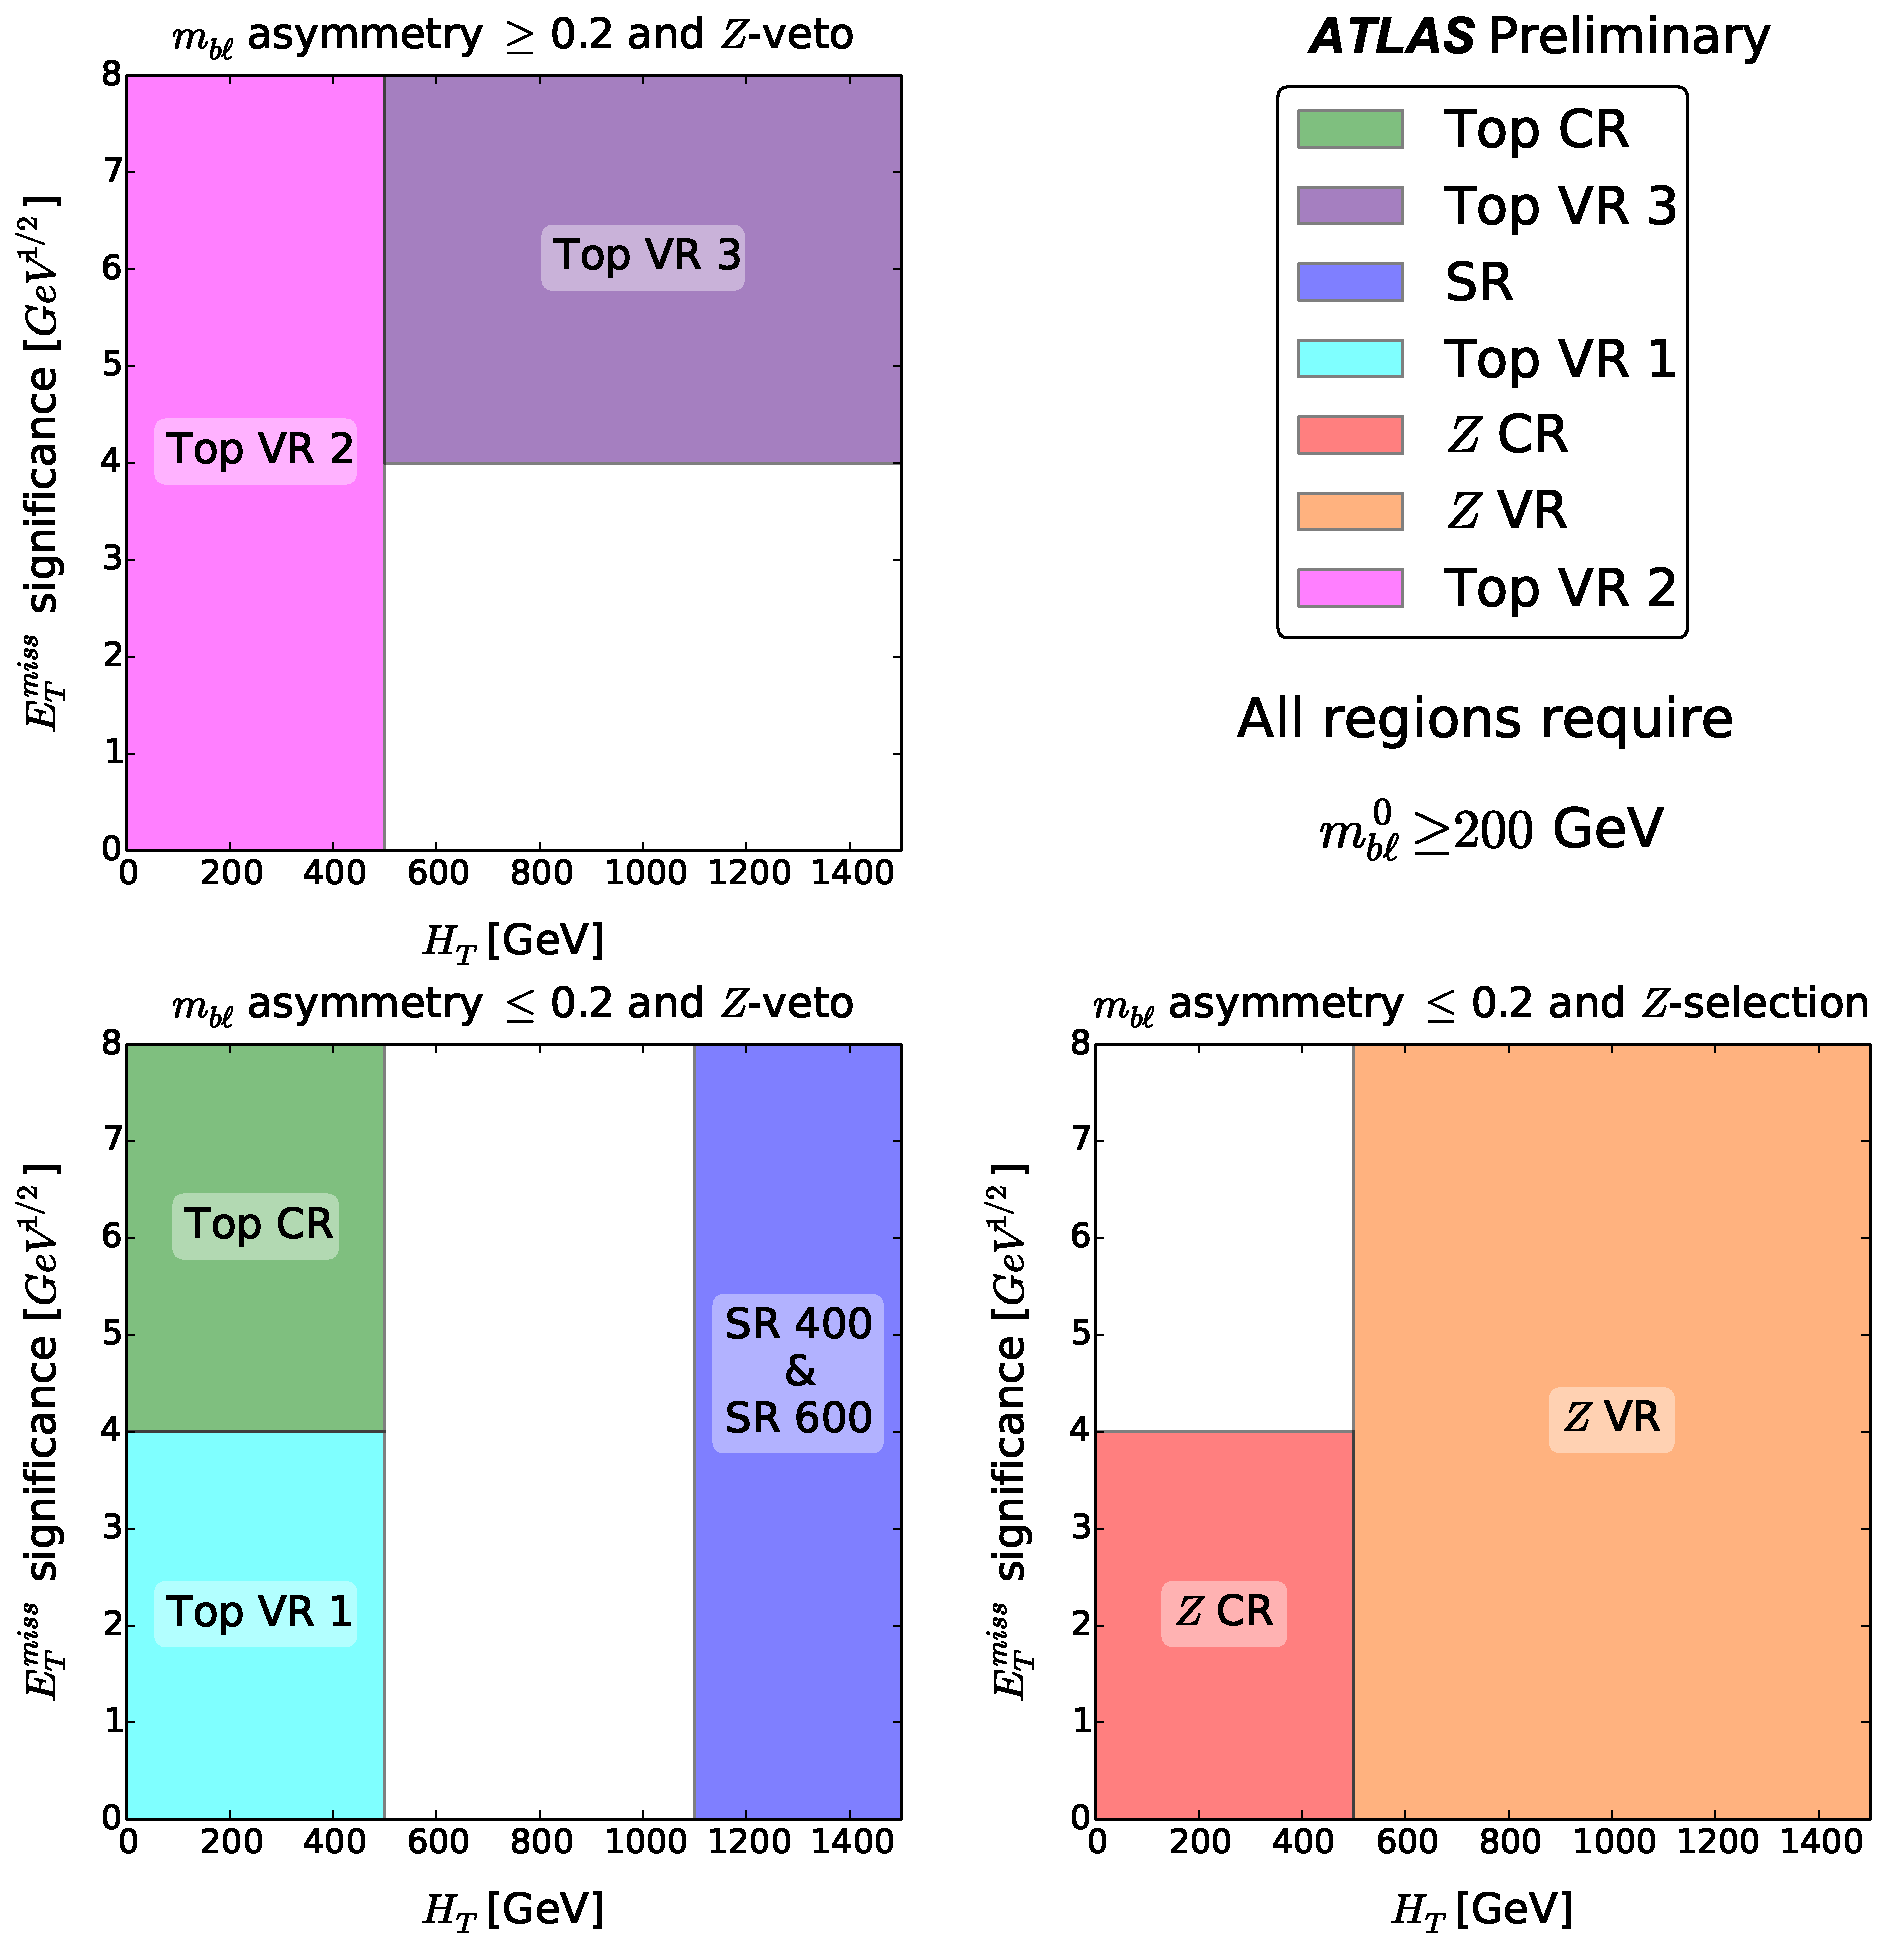
\includegraphics[width=0.6\textwidth]{figs/blstop/regions__met_sig__ht_plane.pdf}
  \caption{Position of the regions in the \METSIG\ versus \HT\ space. The two
    left plots show the \METSIG-\HT~plane after requiring the invariant mass
    of the two leptons is not consistent with the Z boson, with the top plot
    requiring $\MBLASYM \geq 0.2$ and the bottom requiring $\MBLASYM \leq 0.2$.
    The right plot shows the plane when requiring the invariant mass of the
    two leptons is consistent with the Z boson, and the leptons are of the
    same flavor. The two SRs apply a different requirement on the
    invariant mass of the higher-mass $b\ell$ pair. SR~400 requires
    $\MBL^{0} \geq 400$ \GeV, and SR~600 requires $\MBL^{0} \geq 600$ \GeV.
  }
  \label{fig:region_coverage}
\end{figure}

The \HT, \MBLASYM, and $\MBL^0$ distributions are shown in
Figure~\ref{fig:n_minus_one_sr} for the simulated background processes
and three signal models.  In this figure, all the SR
selections apart from that on the variable being shown are applied.
The number of expected signal events (for the same three signal models)
passing each selection requirement is shown in Table~\ref{tab:sr_cutflow}.
The estimates shown in Figure \ref{fig:n_minus_one_sr} and
Table~\ref{tab:sr_cutflow} are taken from MC simulation, and the event
yields are normalized to 20.3 \ifb.

\begin{figure}
\centering
\resizebox{0.48\linewidth}{!}{
  \begin{tikzpicture}
  \node[anchor=south west, inner sep=0] (image) at (0,0) {
    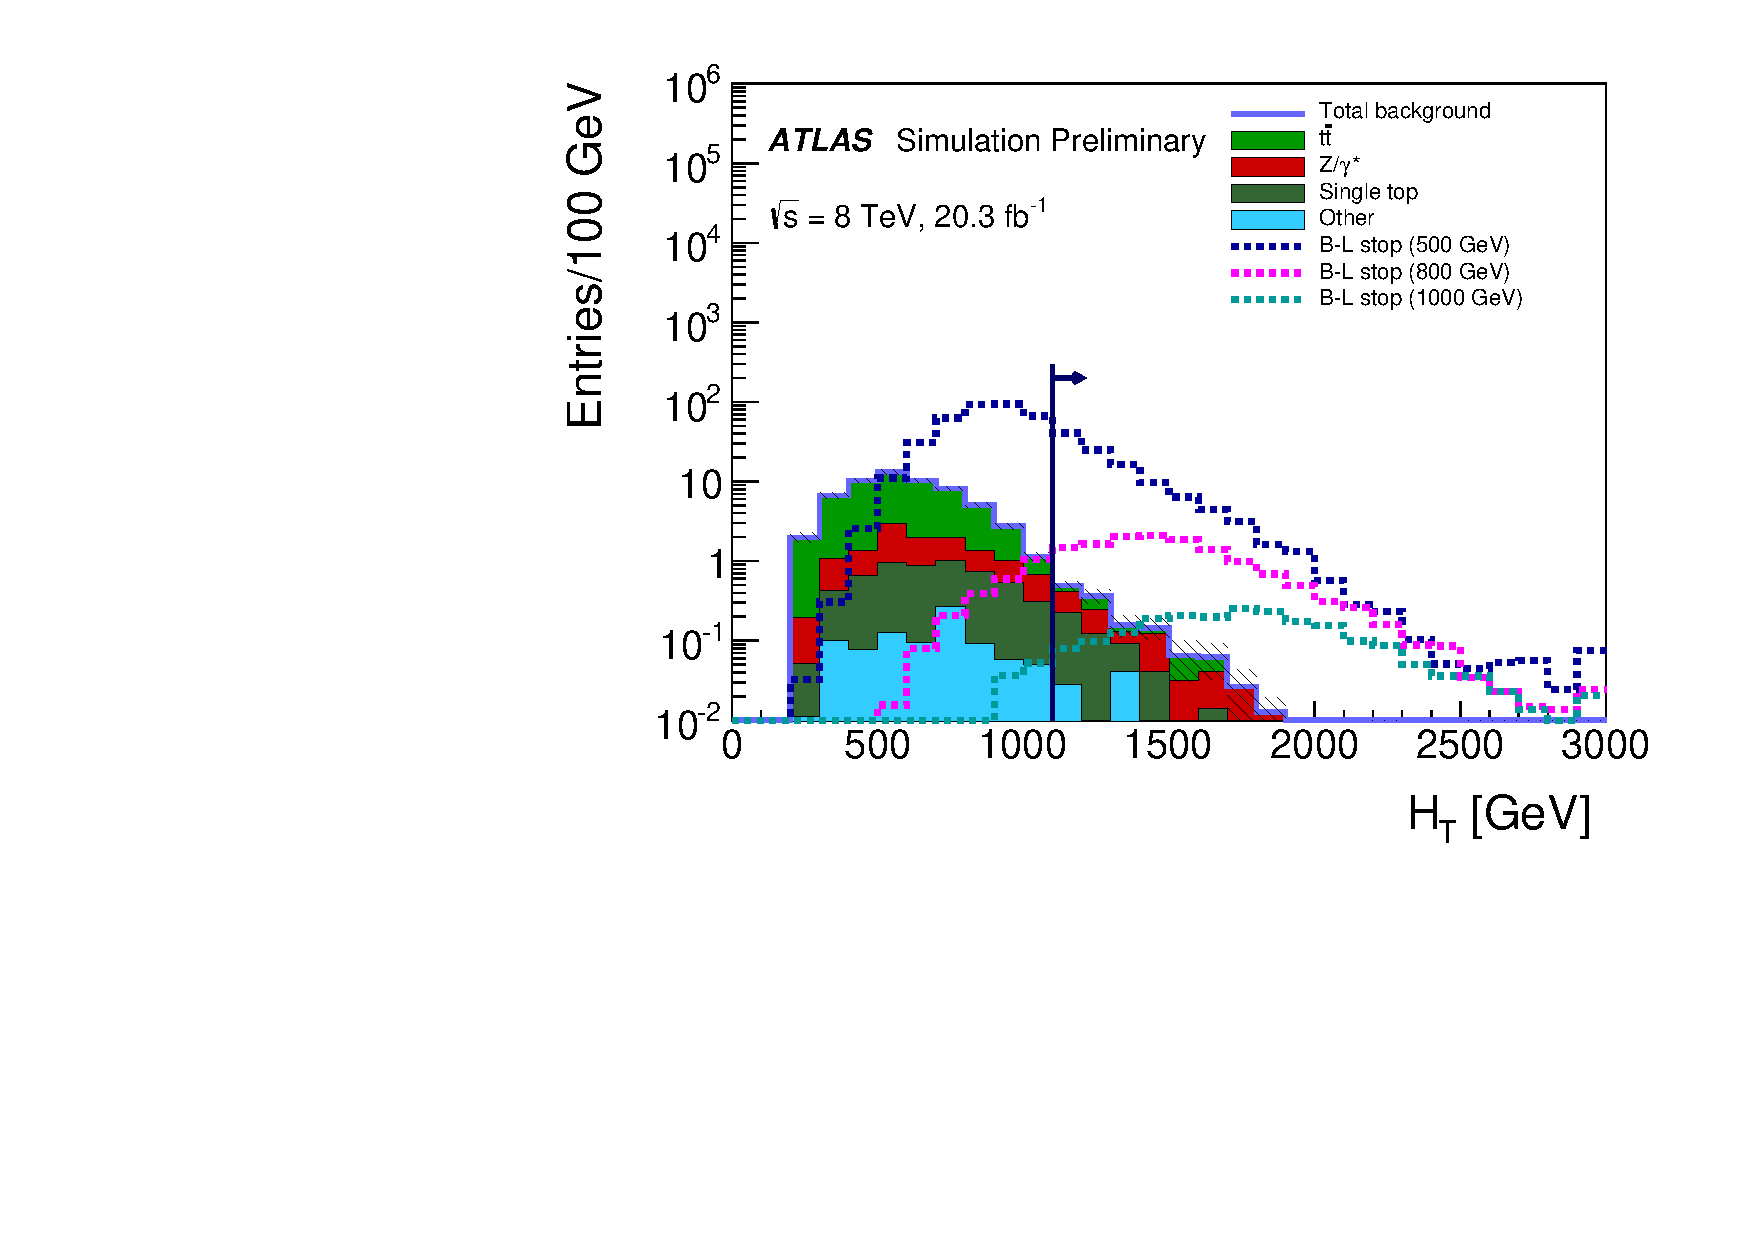
\includegraphics[width=0.48\textwidth]{figs/blstop/ht_sr_400_minus_ht.pdf}
  };
  \end{tikzpicture}
}
%%
\resizebox{0.48\linewidth}{!}{
  \begin{tikzpicture}
  \node[anchor=south west, inner sep=0] (image) at (0,0) {
    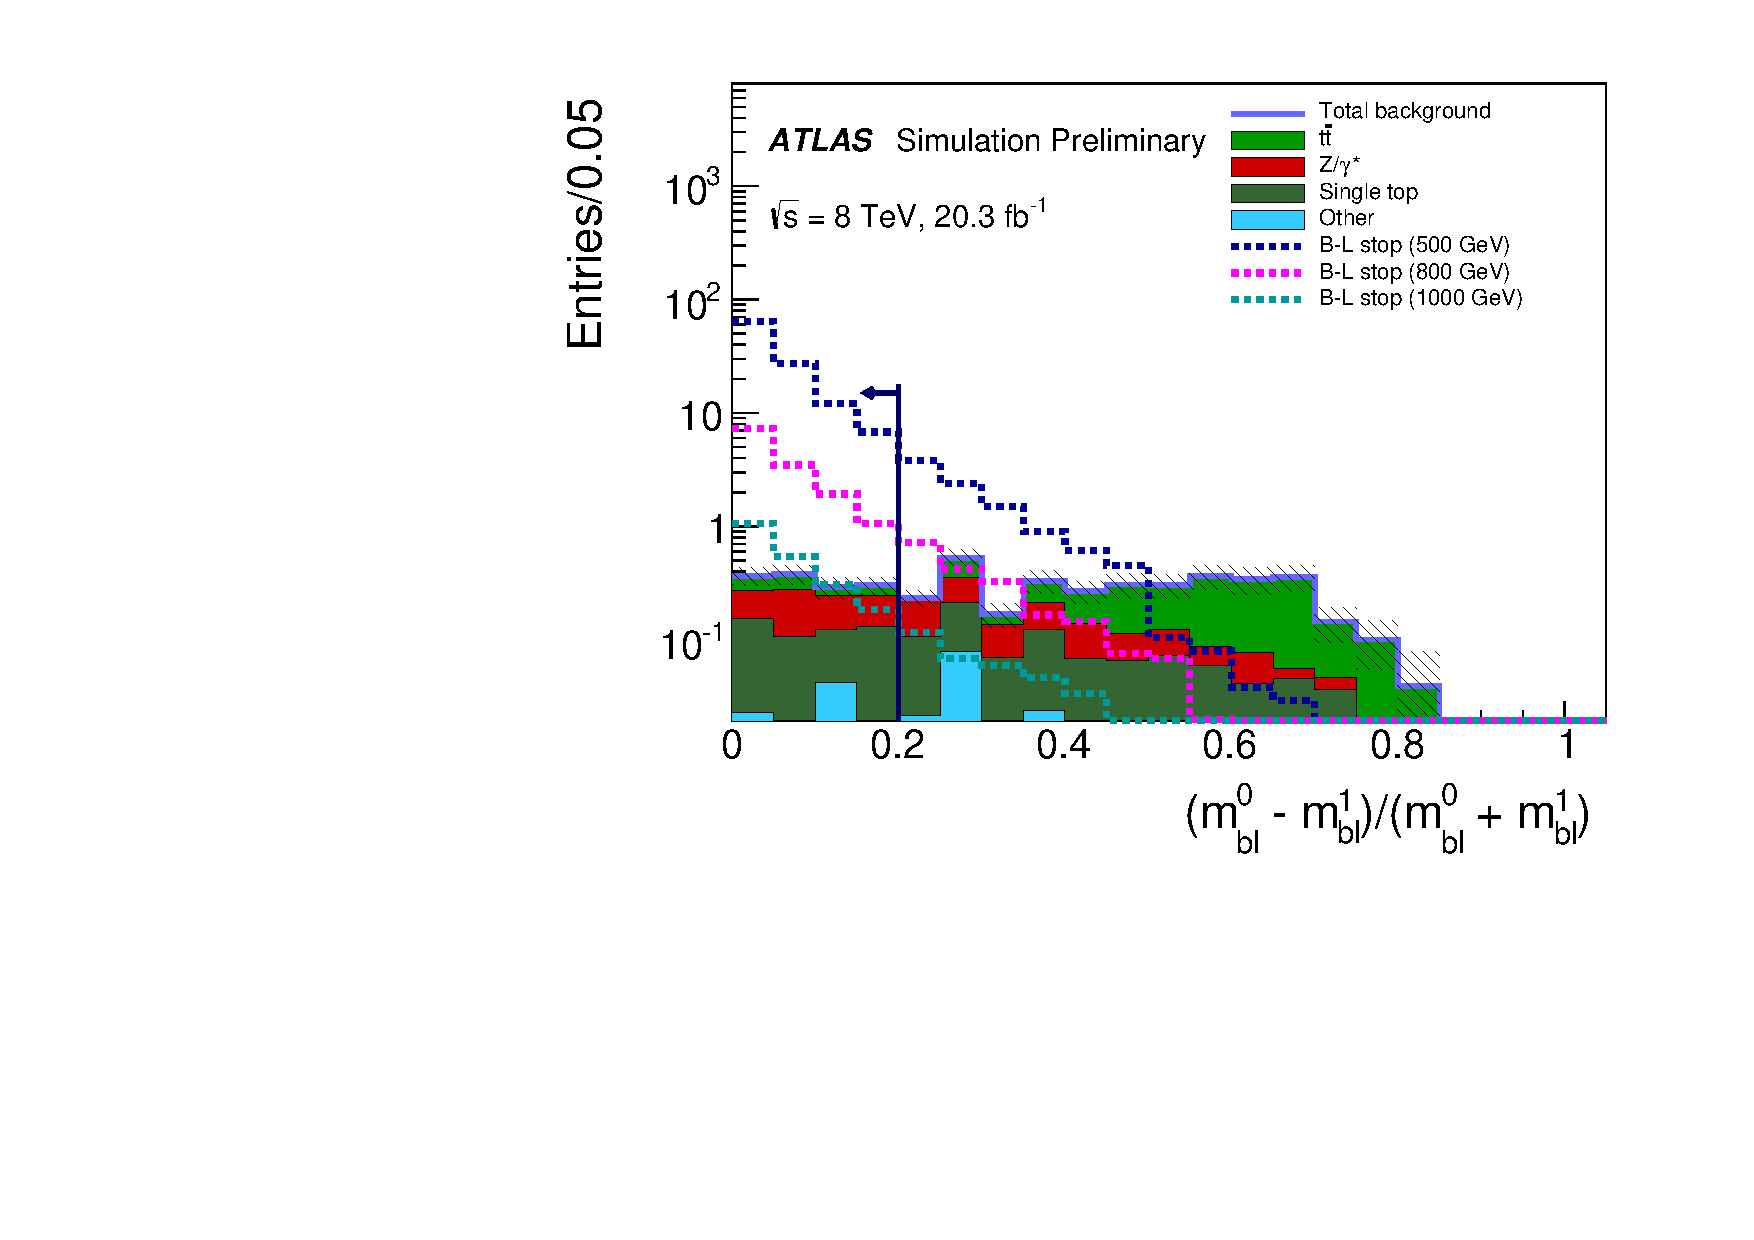
\includegraphics[width=0.48\textwidth]{figs/blstop/mbl_asym_sr_400_minus_mbl_asym.pdf}
  };
  \end{tikzpicture}
}
%%
\resizebox{0.48\linewidth}{!}{
  \begin{tikzpicture}
  \node[anchor=south west, inner sep=0] (image) at (0,0) {
    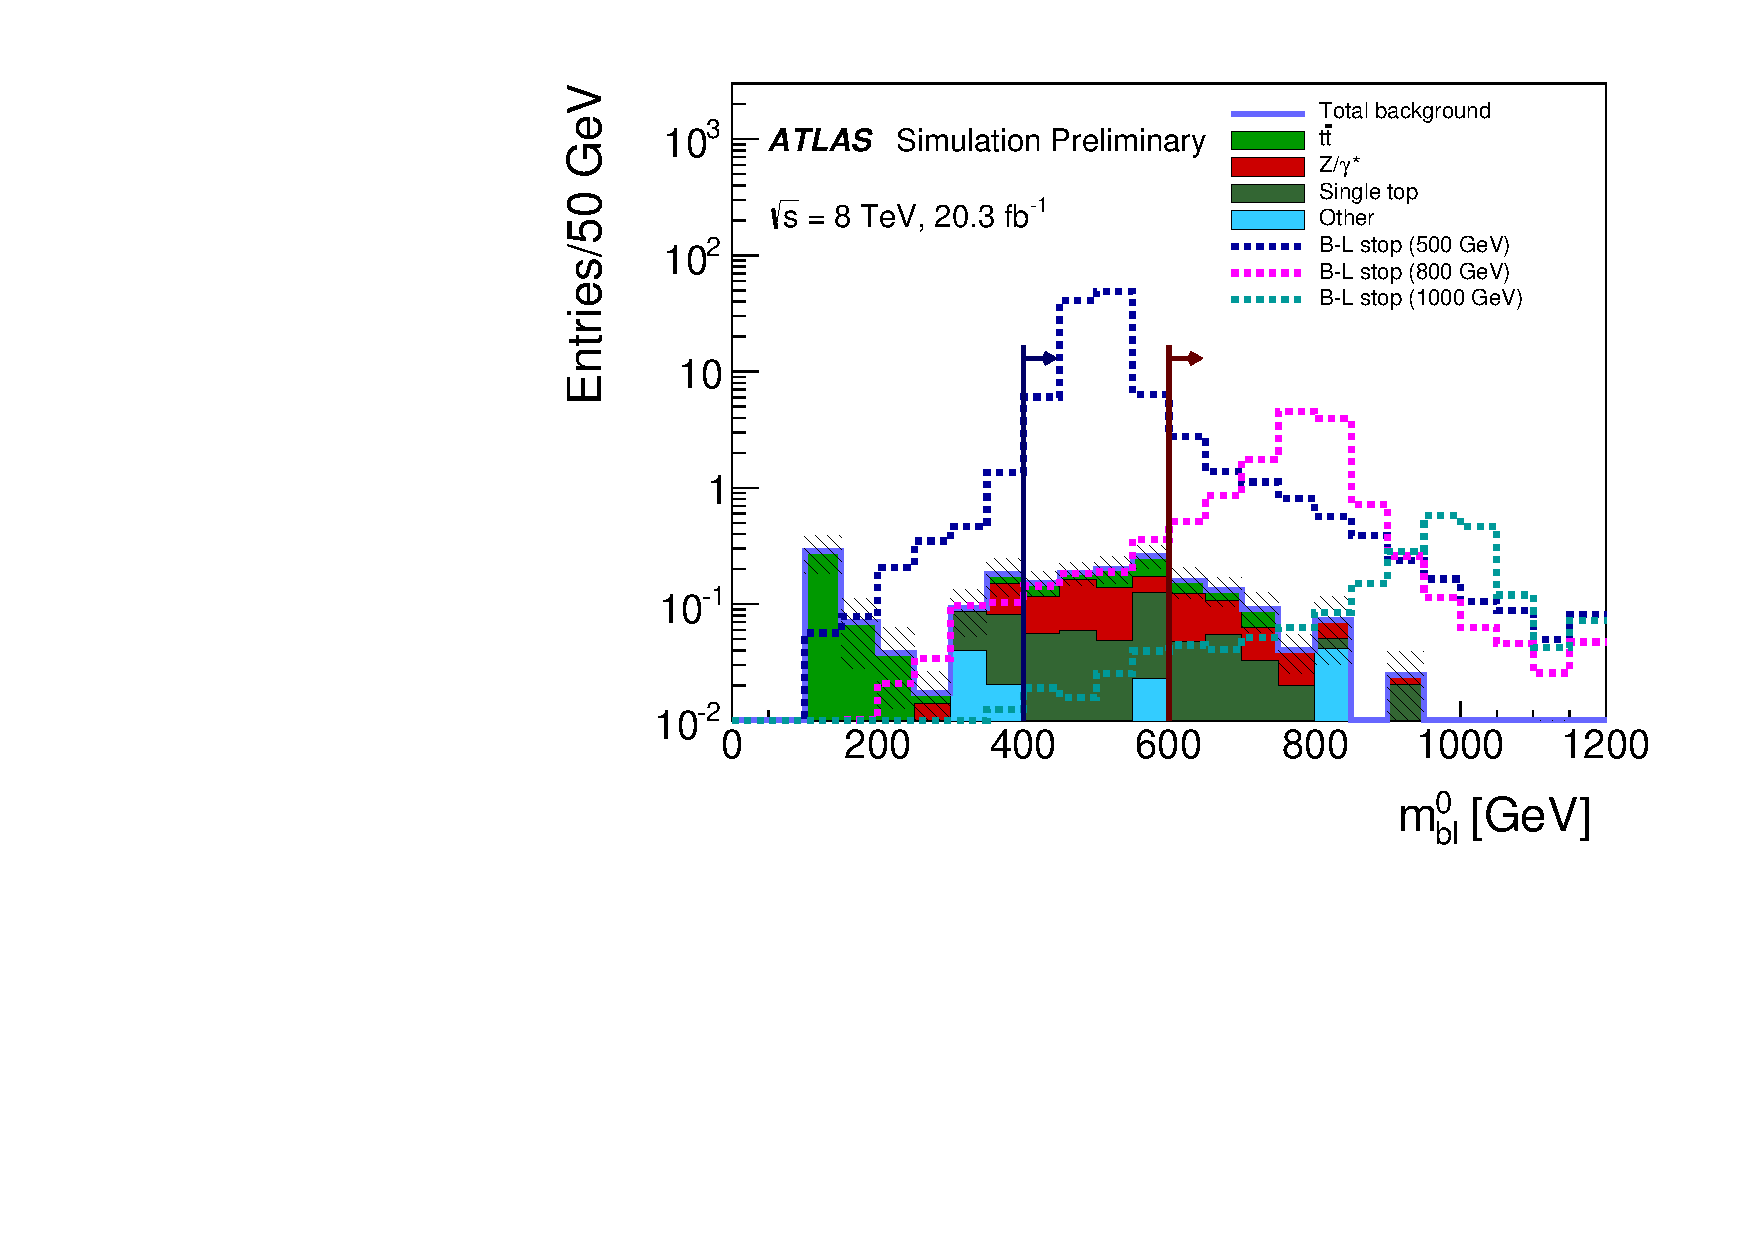
\includegraphics[width=0.48\textwidth]{figs/blstop/mbl_0_sr_minus_mbl.pdf}
  };
  \end{tikzpicture}
}
\caption{Distributions of the variables which are used to define the
  SRs. These plots show the MC simulated background samples and
  three signal models, and are made after applying all the SR
  selection criteria except for that on the variable shown. The top
  two plots show the \HT\ and \MBLASYM\ variables, and the bottom plot shows
  the $\MBL^0$ distribution.
  The arrows show the SR requirement on the variable being shown.
  In each plot, the last bin includes the overflow for values beyond the
  maximum shown. The hashed error bands show only the statistical
  uncertainty on the background MC simulation samples. The signal
  models have an assumed
  $Br(\tilde{t}\rightarrow be) = Br(\tilde{t}\rightarrow b\mu) = 0.5$.
}
\label{fig:n_minus_one_sr}
%%
\end{figure}

\begin{table}[ht]
  \caption{The number of expected signal events pasing each of the signal
    region cuts. This is shown for stop masses of 500~\GeV, 800~\GeV, and
    1000~\GeV.  The estimated yields are taken from MC simulation,
    and are normalized to 20.3~\ifb, and the uncertainty given is the
    MC statistical uncertainty. The signal models have an assumed
    branching fraction of
    $Br(\tilde{t}\rightarrow be) = Br(\tilde{t}\rightarrow b\mu) = 0.5$.
  }
  \label{tab:sr_cutflow}
  %
  \centering{
    \begin{tabular}{l|ccc}
      \toprule
      Selection                       & $m_{\tilde{t}} = 500~\GeV$ & $m_{\tilde{t}} = 800~\GeV$ & $m_{\tilde{t}} = 1000~\GeV$ \\
      \midrule
      $\sigma \cdot L$                & $1750 \pm 260$             & $59 \pm 12$                & $8.9 \pm 2.5$ \\
      \midrule
      $bb\ell\ell$                    & $624 \pm 4$                & $19.65 \pm 0.18$           & $2.68 \pm 0.05$   \\
      $Z$ veto                        & $619 \pm 4$                & $19.62 \pm 0.18$           & $2.68 \pm 0.05$   \\
      $H_{T} \ge$~1100 \GeV           & $122.9 \pm 1.8$            & $16.01 \pm 0.17$           & $2.50 \pm 0.04$   \\
      $m_{b\ell}$ asymmetry $\leq 0.2$ & $112.8 \pm 1.7$            & $14.00 \pm 0.15$           & $2.11 \pm 0.04$   \\
      \midrule
      $m_{b\ell} \geq 400$ \GeV        & $110.3 \pm 1.7$            & $13.74 \pm 0.15$           & $2.09 \pm 0.04$   \\
      $m_{b\ell} \geq 600$ \GeV        & $7.7 \pm 0.4$              & $12.86 \pm 0.15$           & $1.99 \pm 0.04$   \\
      \bottomrule
    \end{tabular}
  }
\end{table}

%% -----------------------------------------------------------------------------
\section{Background estimate}
\label{sec:bkg}

The background estimates of the $t\bar{t}$ and the $Z/\gamma^{*}$+jets
backgrounds use MC simulation normalized in dedicated data
control regions (CRs), the top control region (Top CR) and $Z$ control
region ($Z$ CR) respectively.  The remaining backgrounds are estimated using
simulation. Several validation regions (VRs) are
defined to validate the extrapolation from the CRs to regions with different
kinematics.

Both the Top CR and $Z$ CR require \HT\ to be less than or equal to
500~\GeV\ to reduce the amount of
signal contamination in the regions. A cut of $\MBLASYM \leq 0.2$ is applied to
match the signal regions, and $\MBL^0$ is required to be above 200 \GeV. No
requirement is made on the invariant mass of the second pair.

The \METSIG\ variable is used to define CRs that are relatively pure 
in $t\bar{t}$ or $Z/\gamma^{*}$+jets, where
\begin{equation}
  \METSIG = \frac{\MET}{\sqrt{\HT}}.
\end{equation}
Processes like $t\bar{t}$, with real \MET, tend to have large \METSIG, while
$Z/\gamma^{*}$+jets, where the \MET\ is from mismeasurement, tend to
have low \METSIG. For this reason, the Top CR requires 
$\METSIG \geq 4 \GeV^{1/2}$ and the $Z$ CR requires
$\METSIG \leq 4 \GeV^{1/2}$.  
The definitions of the CRs, and VRs are summarized in
Table~\ref{tab:regions} and Figure~\ref{fig:region_coverage}.

The normalization of the $t\bar{t}$ and the $Z/\gamma^{*}$+jets backgrounds are
determined using a simultaneous fit, which takes into account
cross-contamination of the different background processes between the
CRs as well as the statistical and systematic
uncertainties (described in Section~\ref{sec:systematics})~\cite{Baak:2014wma}.
The remaining background estimates, due to  single top and other SM processes,
are taken from the MC simulation.
The number of observed events as well as the expected number
of events in each of the CRs and VRs are shown in
Table \ref{tab:bkg_only_fit_results}.
The agreement between the observed number of events and the fitted event
yields in the VRs is summarized in Figure \ref{fig:pull_dist_vr}.
Using the fitted backgrounds, the dominant process in the same-flavor
channels of the SRs is $Z/\gamma^{*}$+jets followed by single top and
$t\bar{t}$. In the $e\mu$ channel, the $Z/\gamma^{*}$+jets background does
not contribute, thus, the largest backgrounds are single top and $t\bar{t}$.
As a result of the fit, the $Z/\gamma^{*}$+jets background is scaled up by
approximately 40\%. Due to this large normalization factor, the background is
over-predicted in the $Z$ VR. This over-prediction is taken as an additional
systematic uncertainty, described in Section~\ref{sec:systematics}.

% - - - - - - - - - - - - - - - - - - - - - - - - - - - - - - - - - - - - - - -
\begin{table}[ht]
  \caption{The observed and expected event yields in the CRs and VRs. The
    expected event yields are shown before and after a fit to the data in
    the CRs. The fitted background yields in the CRs match the observed
    number of events in data by construction.
  }
  \label{tab:bkg_only_fit_results}
  %
  \begin{center}
    \begin{tabular}{lrrrrrr}
      \toprule
                                  & Top CR           & Z CR            & Top VR 1       & Top VR 2      & Top VR 3        & Z VR            \\
      \midrule
      Observed                    & $369$            & $327$           & $645$          & $606$         & $67$            & $101$           \\
      \midrule
      Fitted background           & $369   \pm 19$   & $327  \pm 18$   & $690  \pm 50$  & $630 \pm 40$  & $72   \pm 5$    & $130  \pm 60$   \\
      \midrule
      Fitted $t\bar{t}$           & $346   \pm 19$   & $9.1  \pm 0.7$  & $600  \pm 40$  & $497 \pm 35$  & $54   \pm 5$    & $2.99 \pm 0.24$ \\
      Fitted $Z/\gamma^{*}$+jets  & $3.2   \pm 0.5$  & $309  \pm 18$   & $63   \pm 5$   & $64  \pm 5$   & $1.5  \pm 0.8$  & $120  \pm 60$   \\
      Single top                  & $16.7  \pm 2.0$  & $0.83 \pm 0.09$ & $23.0 \pm 2.6$ & $56  \pm 6$   & $14.1 \pm 1.9$  & $0.32 \pm 0.04$ \\
      Other                       & $2.83  \pm 0.27$ & $8.64 \pm 1.0$  & $4.7  \pm 0.4$ & $8.2 \pm 0.8$ & $2.03 \pm 0.27$ & $6.4  \pm 0.7$  \\
      \midrule
      Input SM                  & $330$            & $230$           & $614$          & $557$         & $66$            & $93$            \\
      \midrule
      Input $t\bar{t}$          & $310$            & $8.2$           & $543$          & $447$         & $49$            & $2.7$           \\
      Input $Z/\gamma^{*}$+jets & $2.2$            & $220$           & $44$           & $45$          & $1.1$           & $83$            \\
      Input single top          & $17$             & $0.8$           & $23$           & $57$          & $14$            & $0.30$          \\
      Input other               & $2.8$            & $8.6$           & $4.7$          & $8.2$         & $2.0$           & $6.40$          \\
      \bottomrule
    \end{tabular}
  \end{center}
\end{table}


\begin{figure}[ht]
\centering
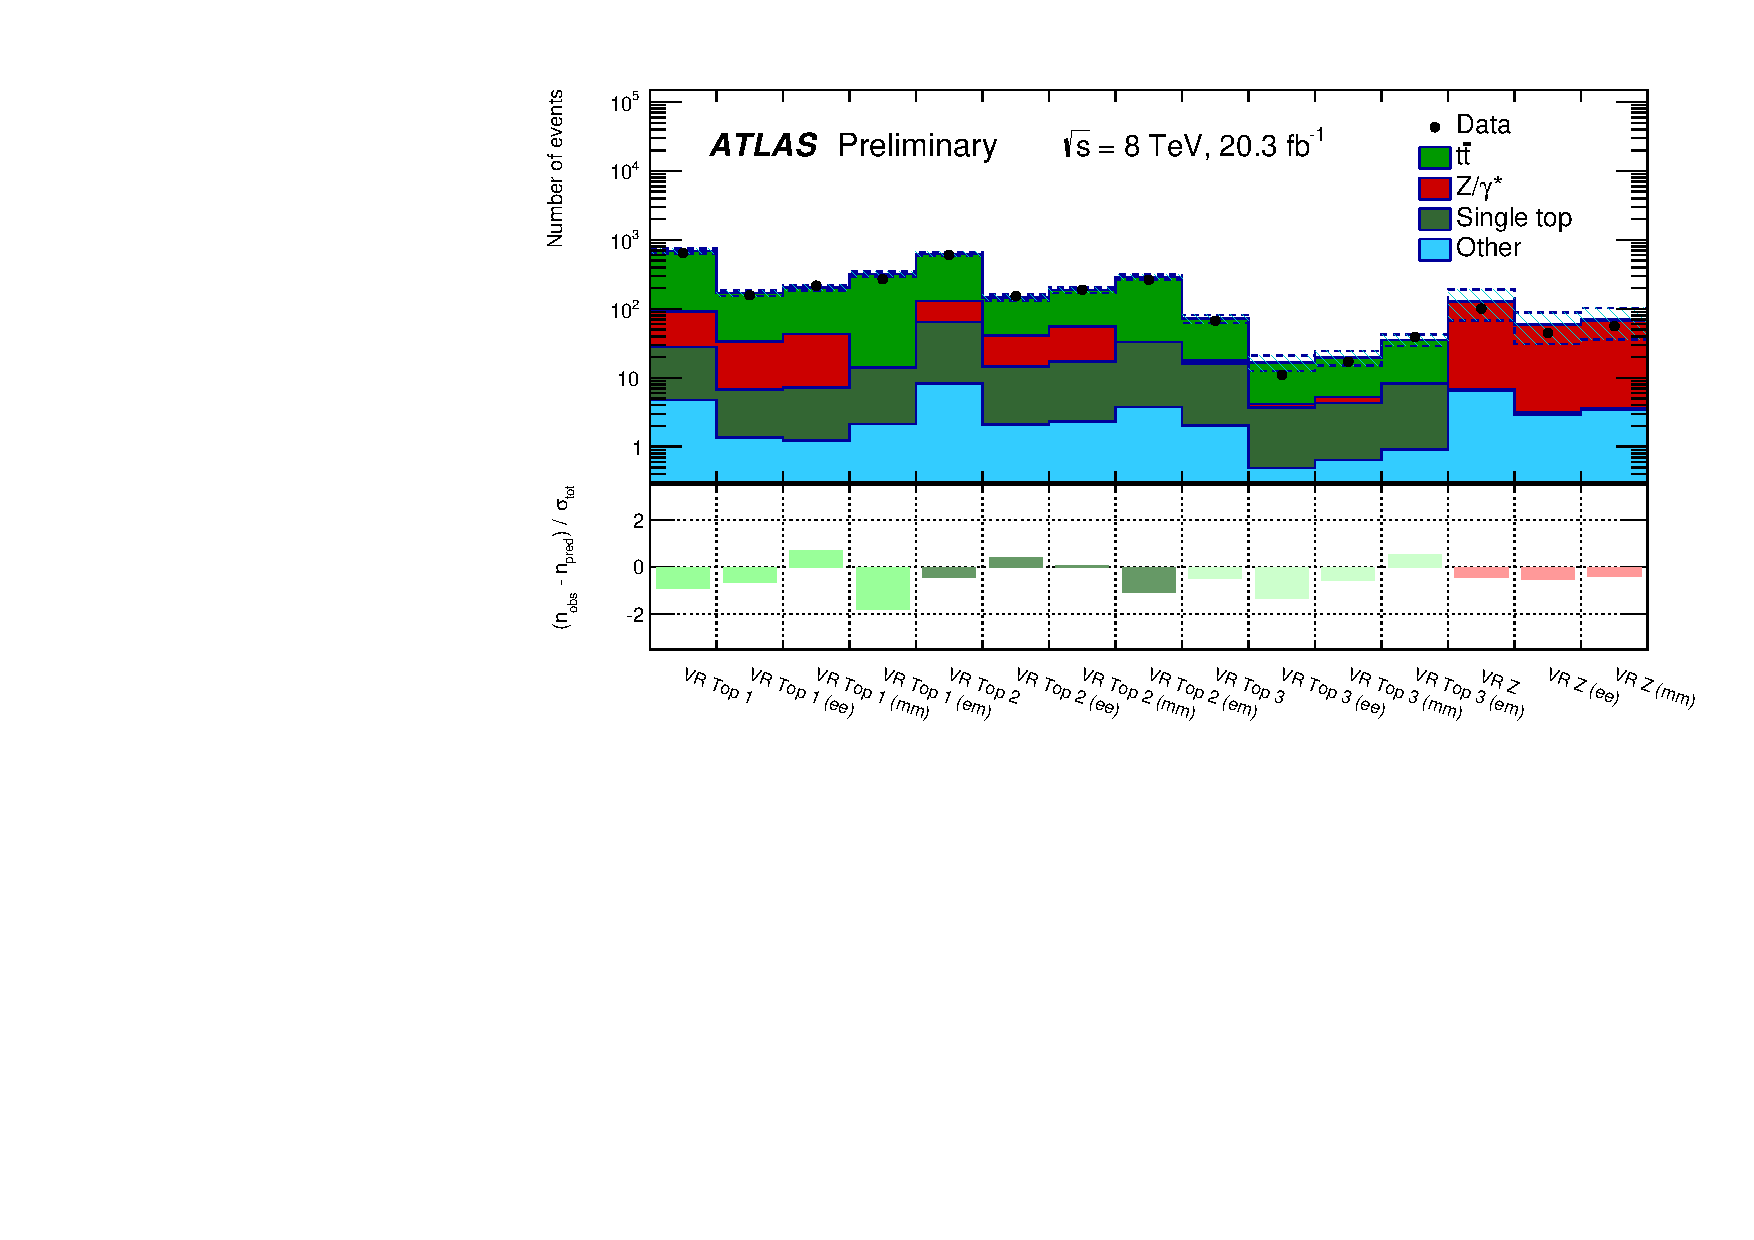
\includegraphics[width=\textwidth]{figs/blstop/histpull_VR_detailed.pdf}
\caption{The top of this plot shows the number of observed and expected
  events in the validation regions, and broken down by flavor channel.
  The uncertainty band includes the statistical uncertainty as well as the
  systematic uncertainty (described in Section~\ref{sec:systematics}). The
  bottom of the plot shows the deviation of that channel's prediction
  from the observed number of events divided by the uncertainty on the
  prediction. The normalization of the background yields are determined
  by fitting the $t\bar{t}$ and $Z/\gamma^{*}$+jets backgrounds to the observed
  data in the two CRs.
}
\label{fig:pull_dist_vr}
\end{figure}

The extrapolation from low \HT\ CRs to the high \HT\ region
where the SRs are located is validated using the Top VR 3
and $Z$ VR. These validation regions show fair
agreement between the observed and predicted event yields as well as
for the shape of the $\MBL^{0}$ and \HT\ distributions as shown in
Figures \ref{fig:mbl_vr} and \ref{fig:ht_vr}.

\begin{figure}
  \centering
  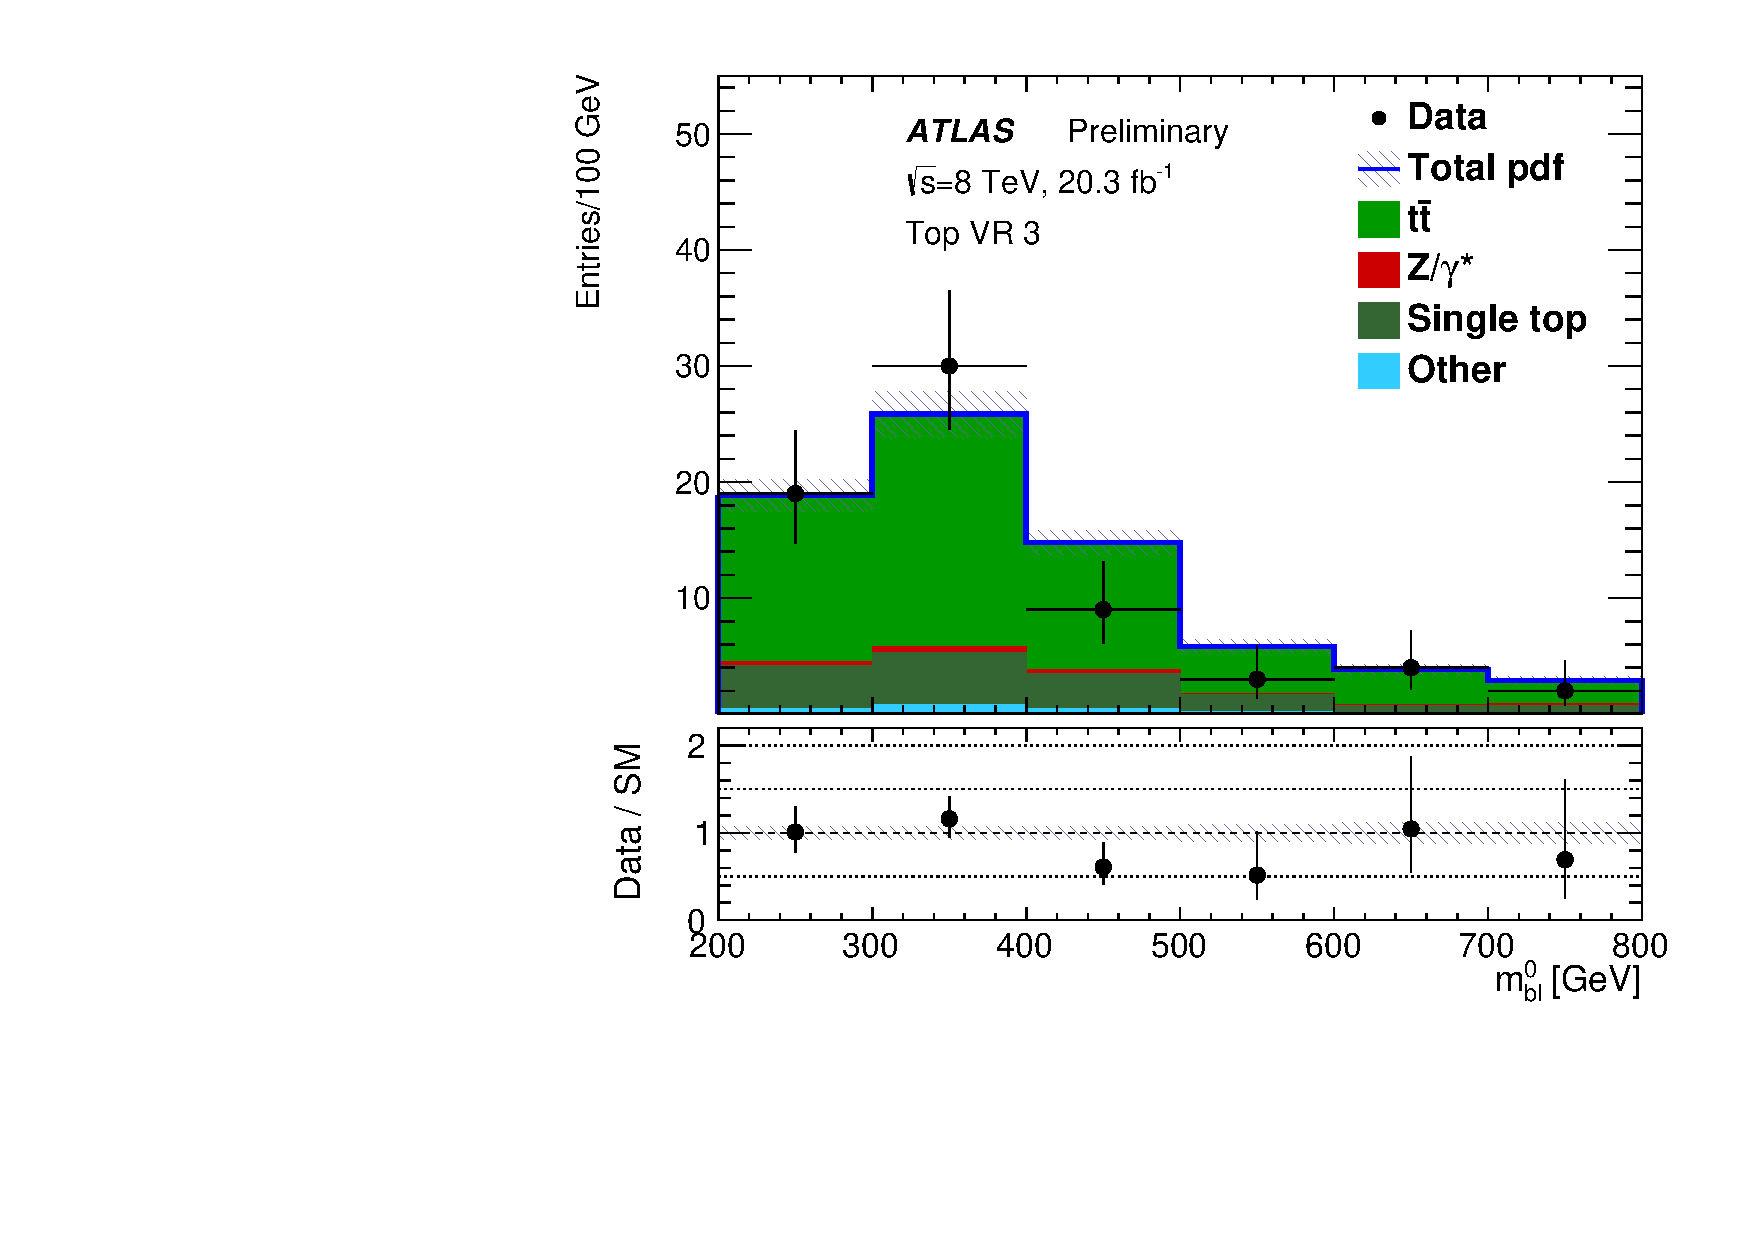
\includegraphics[width=0.48\textwidth]{figs/blstop/vr_top_3_mbl_0.pdf}
  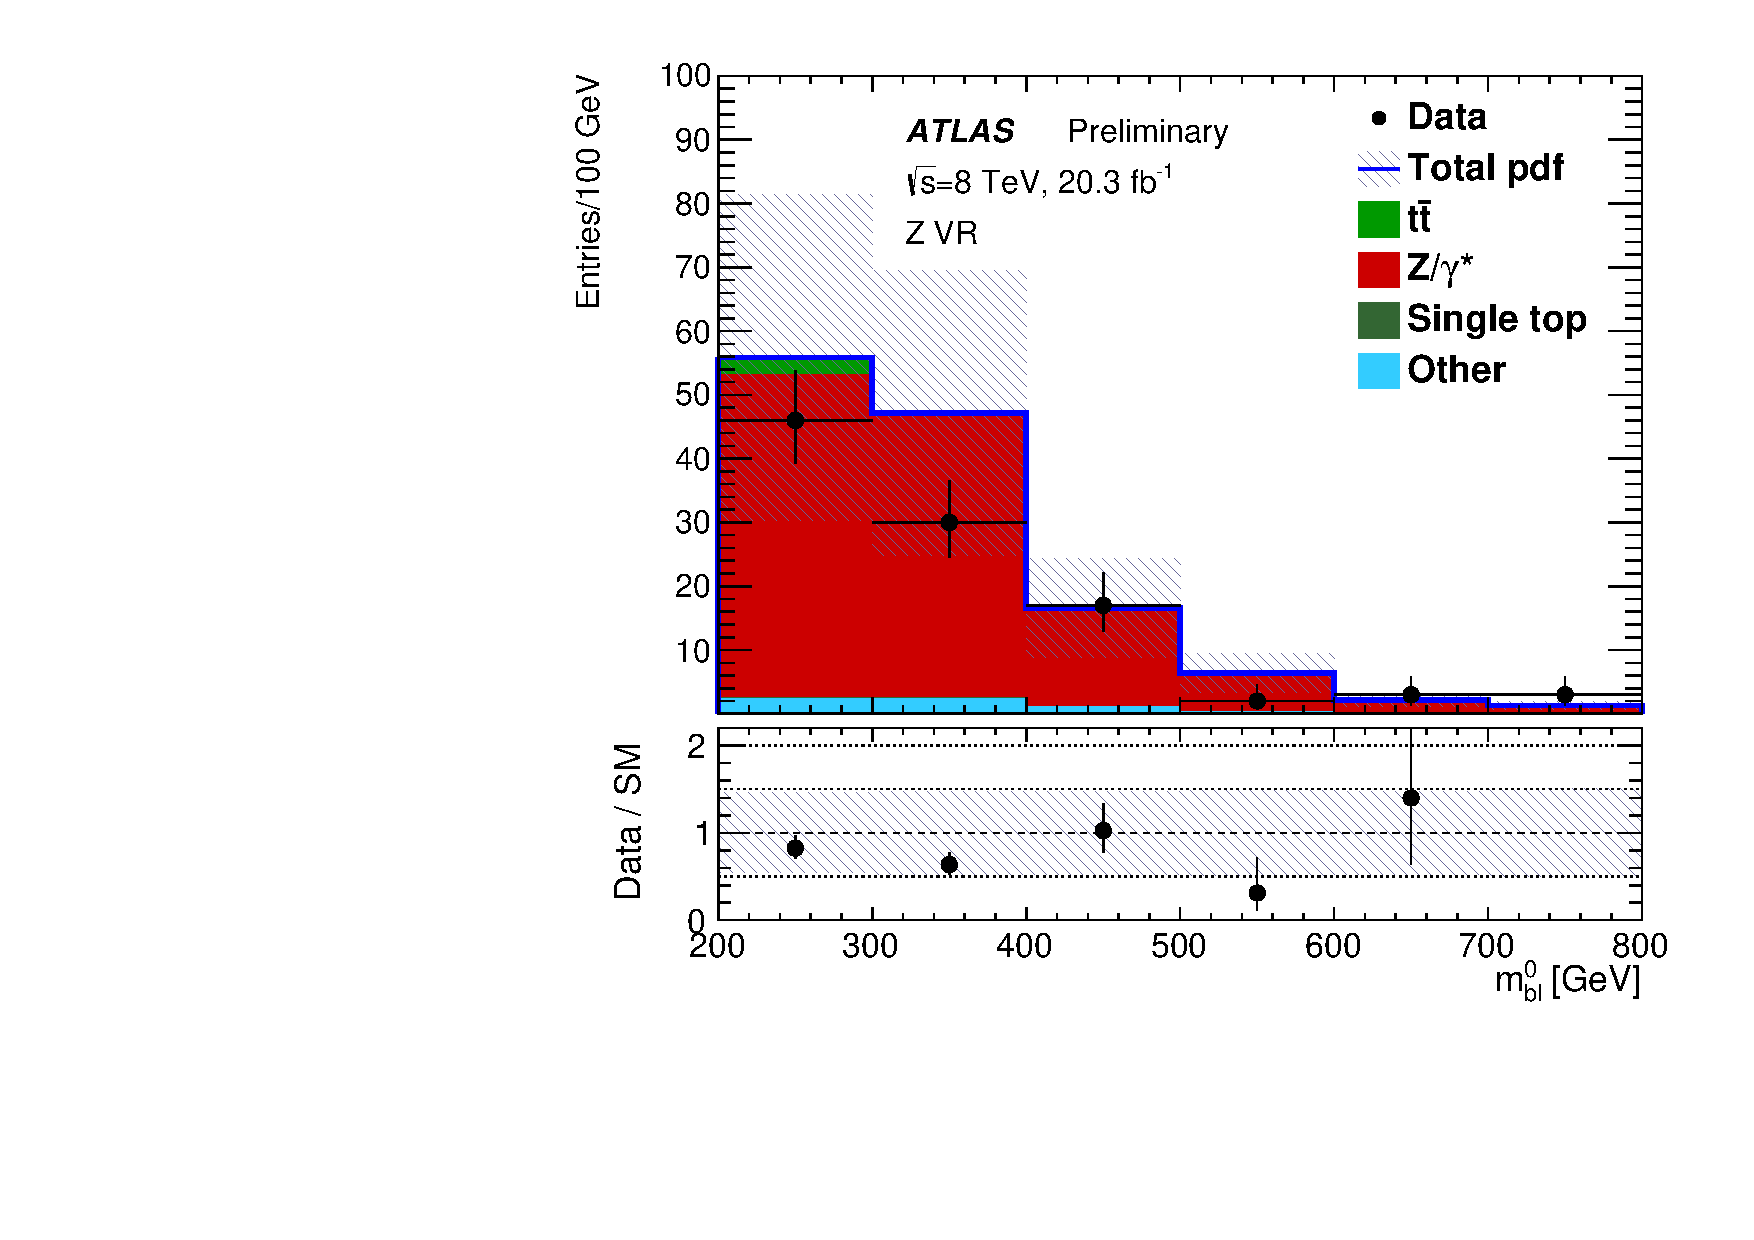
\includegraphics[width=0.48\textwidth]{figs/blstop/vr_Z_mbl_0.pdf}
  \caption{The $\MBL^0$ distribution in Top VR 3 (left)
    and $Z$ VR (right). The Standard Model background prediction is shown
    after setting the normalization of the $t\bar{t}$ and $Z/\gamma^{*}$+jets
    backgrounds based on the observed data in the CRs. The hashed bands show
    the uncertainty on the fitted background prediction including
    all statistical and systematics uncertainties.
    The bottom of each plot shows the ratio of the observed data to the
    Standard Model background prediction.
  }
  \label{fig:mbl_vr}
\end{figure}

\begin{figure}
  \centering
  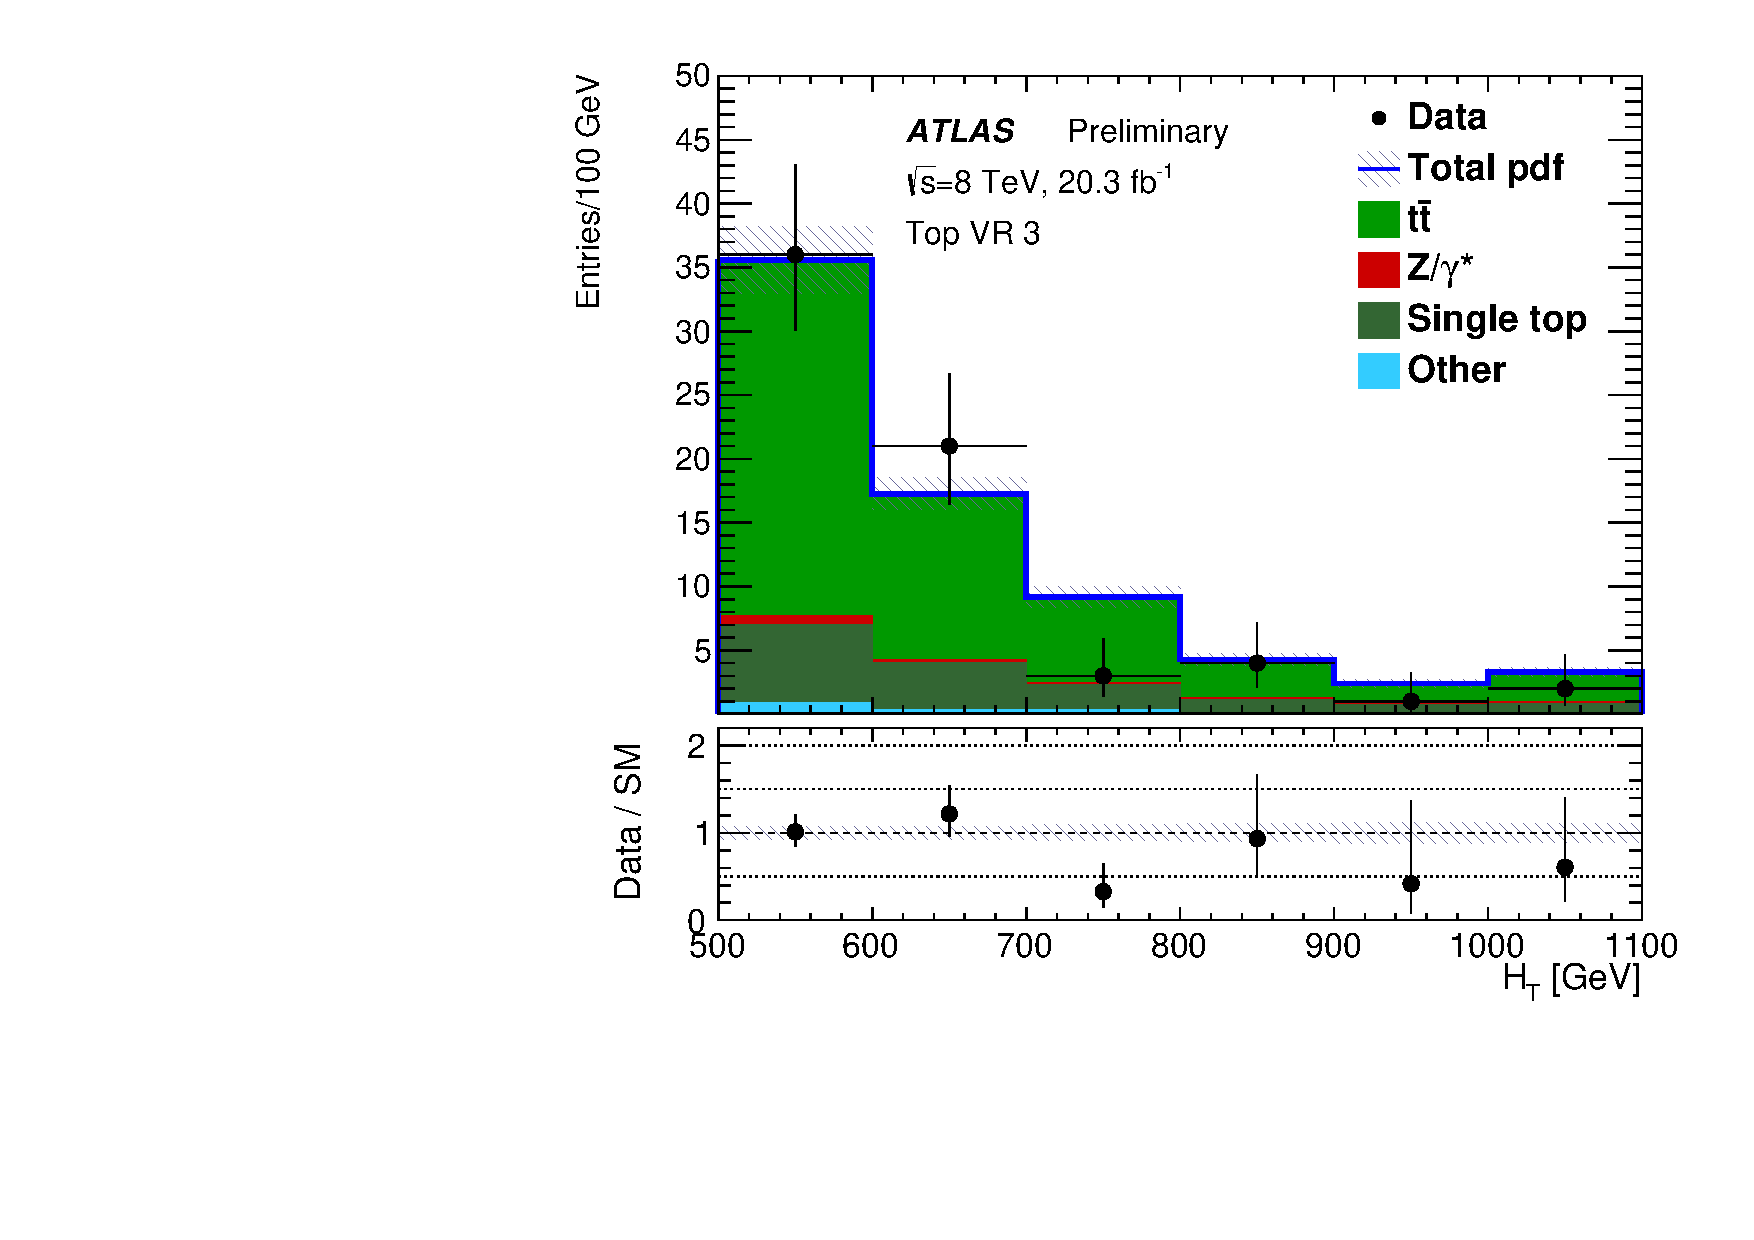
\includegraphics[width=0.48\textwidth]{figs/blstop/vr_top_3_ht_signal.pdf}
  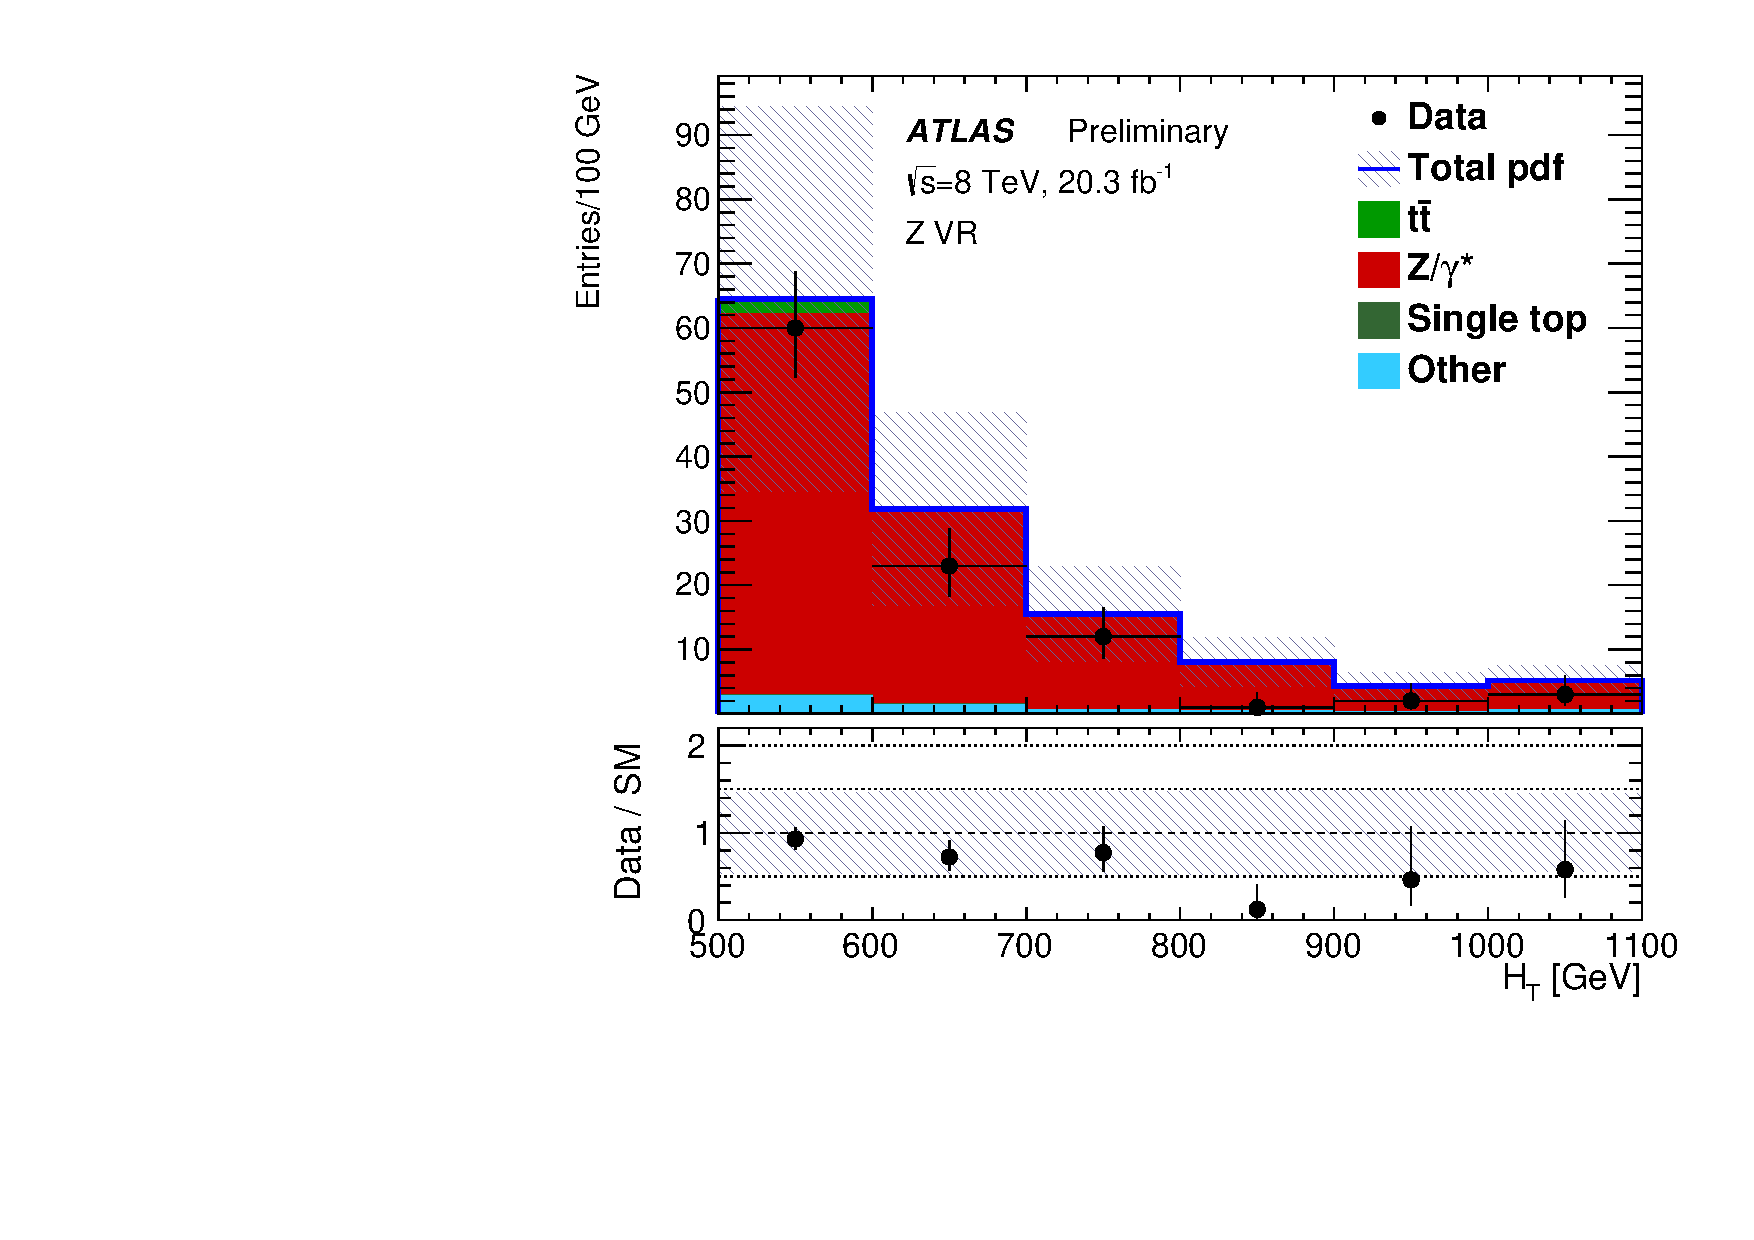
\includegraphics[width=0.48\textwidth]{figs/blstop/vr_Z_ht_signal.pdf}
  \caption{The \HT\ distribution in Top VR 3 (left)
    and $Z$ VR (right). The Standard Model background prediction is shown
    after setting the normalization of the $t\bar{t}$ and $Z/\gamma^{*}$+jets
    backgrounds based on the observed data in the CRs. The hashed bands show
    the uncertainty on the fitted background prediction including
    all statistical and systematics uncertainties.
    The bottom of each plot shows the ratio of the observed data to the
    Standard Model background prediction.
  }
  \label{fig:ht_vr}
\end{figure}

%% -----------------------------------------------------------------------------
\section{Systematic uncertainties}
\label{sec:systematics}

Several sources of systematic uncertainty are considered when determining
the estimated signal and background contributions.
The largest sources of systematic uncertainty are those related to the
MC statistical uncertainty in the SRs, the JES, the $b$-tagging efficiency
and the extrapolation of the $Z/\gamma^{*}$+jets background to high \HT. 
The uncertainty on the lepton energy scale and resolution was considered,
but shown to be negligible.

\begin{itemize}
%%
\item \textbf{Jet energy scale}:
The uncertainty on the JES takes into account the dependence on \pt, $\eta$,
jet flavor, and the number of primary vertices. The components of the JES
uncertainty are varied by $\pm1\sigma$ in the MC simulation and propagated to
the expected event yield.
%%
\item \textbf{$b$-tagging}:
The uncertainty on the $b$-tagging efficiency is evaluated by varying the
correction factors applied to each jet in the simulation within a range that
reflects the systematic uncertainty on the measured tagging and rejection
efficiencies. These uncertainties take into account the dependence on \pt and
jet flavor.
%%
\item \textbf{Jet energy resolution}:
  The uncertainty on the jet energy resolution (JER) is evaluated by
  applying an additional smearing to the \pt of each of the jets in the
  simulation. This smearing is then propagated to the expected event yield.
%%
\item \textbf{\HT\ extrapolation}:
An \HT\ extrapolation uncertainty of 50\% is applied to $Z/\gamma^{*}$+jets
events with $\HT \geq 500$~\GeV. This is assigned to account for
uncertainty on the $Z/\gamma^{*}$+jets \HT\ spectrum. This uncertainty
is derived from the disagreement observed in
Figures~\ref{fig:pull_dist_vr}-\ref{fig:ht_vr}.
%%
\end{itemize}

Several theoretical uncertainties are considered in the modeling of the major
background processes in MC simulation. These include the uncertainty on the
single top ($Wt$) cross section, the uncertainty related to the renormalization
and factorization scales, parton shower, and the limited number of partons
included in the matrix element calculation. These theoretical uncertainties
are on the order of a few percent of the total background prediction. The
uncertainty on the luminosity is assessed for the signal processes, and all
background processes apart from $t\bar{t}$ and $Z/\gamma^{*}$+jets, whose
normalizations are determined using data.
The relative systematic uncertainty on the total background estimate in the
SRs is shown in Table \ref{tab:systematic_breakdown}

\begin{table}[ht]
\caption{Summary of the effect of each considered sources of systematic
  uncertainty on the background estimate in SR~400 and SR~600. Several
  sources of theoretical systematic uncertainty which have a small
  effect on the total background estimate are grouped into the
  ``Other theory'' category.
}
\label{tab:systematic_breakdown}
%
\centering{
  \begin{tabular}{lcc}
  \toprule
    Systematic &
    \multirow{2}{*}{SR~400} &
    \multirow{2}{*}{SR~600} \\
    Uncertainty (\%) \\
    \midrule
    JES                          & 15     & 3  \\
    $b$-tagging                  & 13     & 12 \\
    JER                          & 5      & 1  \\
    Luminosity                   & 1      & 1  \\
    \midrule                                   
    \HT\ extrapolation           & 19     & 20 \\
    MC statistical               & 13     & 23 \\
    CR statistical               & 3      & 3 \\
    $Wt$ cross section           & 2      & 2  \\
    Other theory                 & 1      & 2  \\
    \bottomrule
    \end{tabular}
}
\end{table}

For each of the signal models, the effects of uncertainty on the JES,
$b$-tagging efficiency, JER, and luminosity are considered as well as the
uncertainty on the signal model cross section which ranges between 14\%
and 28\%.

%% -----------------------------------------------------------------------------
\section{Results}
\label{sec:results}

The background yields in these signal regions are determined by a
maximum likelihood fit~\cite{Baak:2014wma} for the $t\bar{t}$ and
$Z/\gamma^{*}$+jets
normalizations, which are constrained by the observed data in the Top
and $Z$ control regions.  The systematic uncertainties described
previously are included as Gaussian-distributed nuisance parameters.
The fitted background yields and the observed number of events in each
signal region are shown in Tables~\ref{tab:event_yields_sr_400} and
\ref{tab:event_yields_sr_600}. Two events are observed, in agreement with
the Standard Model prediction.  The kinematics of the two selected events
are shown in Table~\ref{tab:sr_event_kinematics}, the $\MBL^0$ and
\HT\ distributions in SR 400 are shown in Figure~\ref{fig:sr_dists}.

\begin{table}
  \caption{The expected and observed event yields in SR~400. The expected event
    yields are shown before and after performing the fit to the data in the
    control regions.
    The last three rows show the model-independent 95\% CL on
    the visible cross section and the number of events (expected and observed)
    in SR~400 from a generic non-Standard Model process.
  }
  \label{tab:event_yields_sr_400}
  %
  \begin{center}
    \begin{tabular}{lrrrr}
      \toprule
                                    & SR~400                & SR~400 $ee$           & SR~400 $\mu\mu$       & SR~400 $e\mu$  \\
      \midrule
      Observed                      & $2$                   & $0$                   & $2$                   & $0$                \\
      \midrule
      Fitted background             & $1.39 \pm 0.35$       & $0.36 \pm 0.15$       & $0.57 \pm 0.20$       & $0.45 \pm 0.11$    \\
      \midrule
      Fitted $t\bar{t}$             & $0.33 \pm 0.09$       & $0.07 \pm 0.08$       & $0.07 \pm 0.02$       & $0.19 \pm 0.05$    \\
      Fitted $Z/\gamma^{*}$+jets    & $0.54 \pm 0.28$       & $0.20 \pm 0.10$       & $0.35 \pm 0.18$       & $\leq 0.01$    \\
      Single Top                    & $0.44 \pm 0.08$       & $0.10 \pm 0.03$       & $0.11 \pm 0.03$       & $0.23 \pm 0.05$    \\
      Other                         & $0.07 \pm 0.04$       & $\leq 0.01$           & $0.04 \pm 0.02$       & $0.03 \pm 0.03$    \\
      \midrule
      Input SM                      & $1.2$                 & $0.30$                & $0.46$                & $0.43$             \\
      \midrule
      Input $t\bar{t}$              & $0.30$                & $0.06$                & $0.06$                & $0.17$             \\
      Input $Z/\gamma^{*}$+jets     & $0.38$                & $0.14$                & $0.24$                & $0.00$             \\
      Input single Top              & $0.44$                & $0.10$                & $0.11$                & $0.23$             \\
      Input other                   & $0.07$                & $0.00$                & $0.04$                & $0.03$             \\
      \midrule
      $\sigma_\mathrm{vis}$~[fb]    & $0.23$                & $0.11$                & $0.26$                & $0.11$                \\
      Observed $N_\mathrm{non-SM}$  & $4.8$                 & $2.2$                 & $5.4$                 & $2.3$                 \\
      Expected $N_\mathrm{non-SM}$  & ${4.0}^{+2.2}_{-1.1}$ & ${3.2}^{+1.7}_{-1.1}$ & ${3.6}^{+1.9}_{-1.5}$ & ${3.3}^{+1.8}_{-1.3}$ \\
      \bottomrule
    \end{tabular}
  \end{center}
\end{table}

\begin{table}
  \caption{The expected and observed event yields in SR~600. The expected event
    yields are shown before and after performing the fit to the data in the
    control regions.  The last three rows show the model-independent 95\% CL on
    the visible cross section and the number of events (expected and observed)
    in SR~600 from a generic non-Standard Model process.
  }
  \label{tab:event_yields_sr_600}
  %
  \begin{center}
    \begin{tabular}{lrrrr}
      \toprule
                                     & SR~600                & SR~600 $ee$           & SR~600 $\mu\mu$       & SR~600 $e\mu$   \\
      \midrule
      Observed                       & $1$                   & $0$                   & $1$                   & $0$              \\
      \midrule
      Fitted background              & $0.55 \pm 0.15$       & $0.15 \pm 0.06$       & $0.24 \pm 0.10$       & $0.16 \pm 0.06$  \\
      \midrule
      Fitted $t\bar{t}$              & $0.10 \pm 0.02$       & $0.03 \pm 0.01$       & $\leq 0.01$           & $0.07 \pm 0.03$  \\
      Fitted $Z/\gamma^{*}$+jets     & $0.23 \pm 0.12$       & $0.08 \pm 0.05$       & $0.15 \pm 0.08$       & $\leq 0.01$  \\
      Single Top                     & $0.18 \pm 0.04$       & $0.03 \pm 0.01$       & $0.05 \pm 0.02$       & $0.09 \pm 0.03$  \\
      Other                          & $0.04 \pm 0.01$       & $\leq 0.01$           & $0.04 \pm 0.02$       & $\leq 0.01$  \\
      \midrule
      Input SM                       & $0.47$                & $0.12$                & $0.20$                & $0.16$           \\
      \midrule
      Input $t\bar{t}$               & $0.09$                & $0.03$                & $0.00$                & $0.06$           \\
      Input $Z/\gamma^{*}$+jets      & $0.16$                & $0.06$                & $0.10$                & $0.00$           \\
      Input single Top               & $0.18$                & $0.03$                & $0.05$                & $0.09$           \\
      Input other                    & $0.04$                & $0.00$                & $0.04$                & $0.00$           \\
      \midrule
      $\sigma_\mathrm{vis}$~[fb]     & $0.19$                & $0.10$                & $0.20$                & $0.10$                \\
      Observed $N_\mathrm{non-SM}$   & $3.9$                 & $2.1$                 & $4.0$                 & $2.1$                 \\
      Expected $N_\mathrm{non-SM}$   & ${3.5}^{+1.9}_{-1.4}$ & ${2.6}^{+1.6}_{-0.6}$ & ${3.0}^{+1.7}_{-1.0}$ & ${2.7}^{+1.6}_{-0.7}$ \\
      \bottomrule
    \end{tabular}
  \end{center}
\end{table}

\begin{table}
  \caption{The event and object kinematics for the two events passing the
    signal region selection. The first event passes the SR~400 selection
    while the second event passes both SR~400 and SR~600 selections.
  }
  \label{tab:sr_event_kinematics}
  %
  \begin{center}
    \begin{tabular}{lcc}
      \toprule
      Run number                   & 214216    & 210302  \\
      Event number                 & 121272046 & 2292645861 \\
      \midrule
      $\MBL^0$ [\GeV]               & 558       & 686   \\
      %
      $\ell_0$ flavor              & $\mu$     & $\mu$ \\
      $\ell_0$ charge              & $-$       & $-$   \\
      %
      $\ell_0\ p_\mathrm{T}$ [\GeV] & 375       & 272   \\
      $b_0\ p_\mathrm{T}$    [\GeV] & 330       & 460   \\
      %
      $\ell_0\ \eta$               & $-0.11$   & 1.22  \\
      $b_0\ \eta$                  & 0.56      & 0.95  \\
      %
      $\ell_0\ \phi$               & 2.0       & $-1.3$  \\
      $b_0\ \phi$                  & $-2.7$    & 2.5   \\
      %
      \midrule
      $\MBL^1$ [\GeV]               & 526       & 528   \\
      %
      $\ell_1$ flavor              & $\mu$     & $\mu$ \\
      $\ell_1$ charge              & $+$       & $+$     \\
      %
      $\ell_1\ p_\mathrm{T}$ [GeV] & 88        & 96    \\
      $b_1\ p_\mathrm{T}$    [GeV] & 542       & 374   \\
      %
      $\ell_1\ \eta$               & 0.45      & 1.43  \\
      $b_1\ \eta$                  & $-1.1$    & $-0.26$ \\
      %
      $\ell_1\ \phi$               & $-2.3$    & $-0.91$ \\
      $b_1\ \phi$                  & $-0.21$   & 2.3   \\
      %
      \midrule
      \MBLASYM                     & 0.03      & 0.13  \\
      \HT\ [\GeV]                   & 1335      & 1203  \\
      \METSIG\ $[\GeV^{1/2}]$       & 2.9       & 6.4   \\
      \MET\ [\GeV]                  & 107       & 223   \\
      $m_{\ell\ell}$ [\GeV]         & 324       & 71    \\
      \bottomrule
    \end{tabular}
  \end{center}
\end{table}

\begin{figure}[ht]
  \centering
  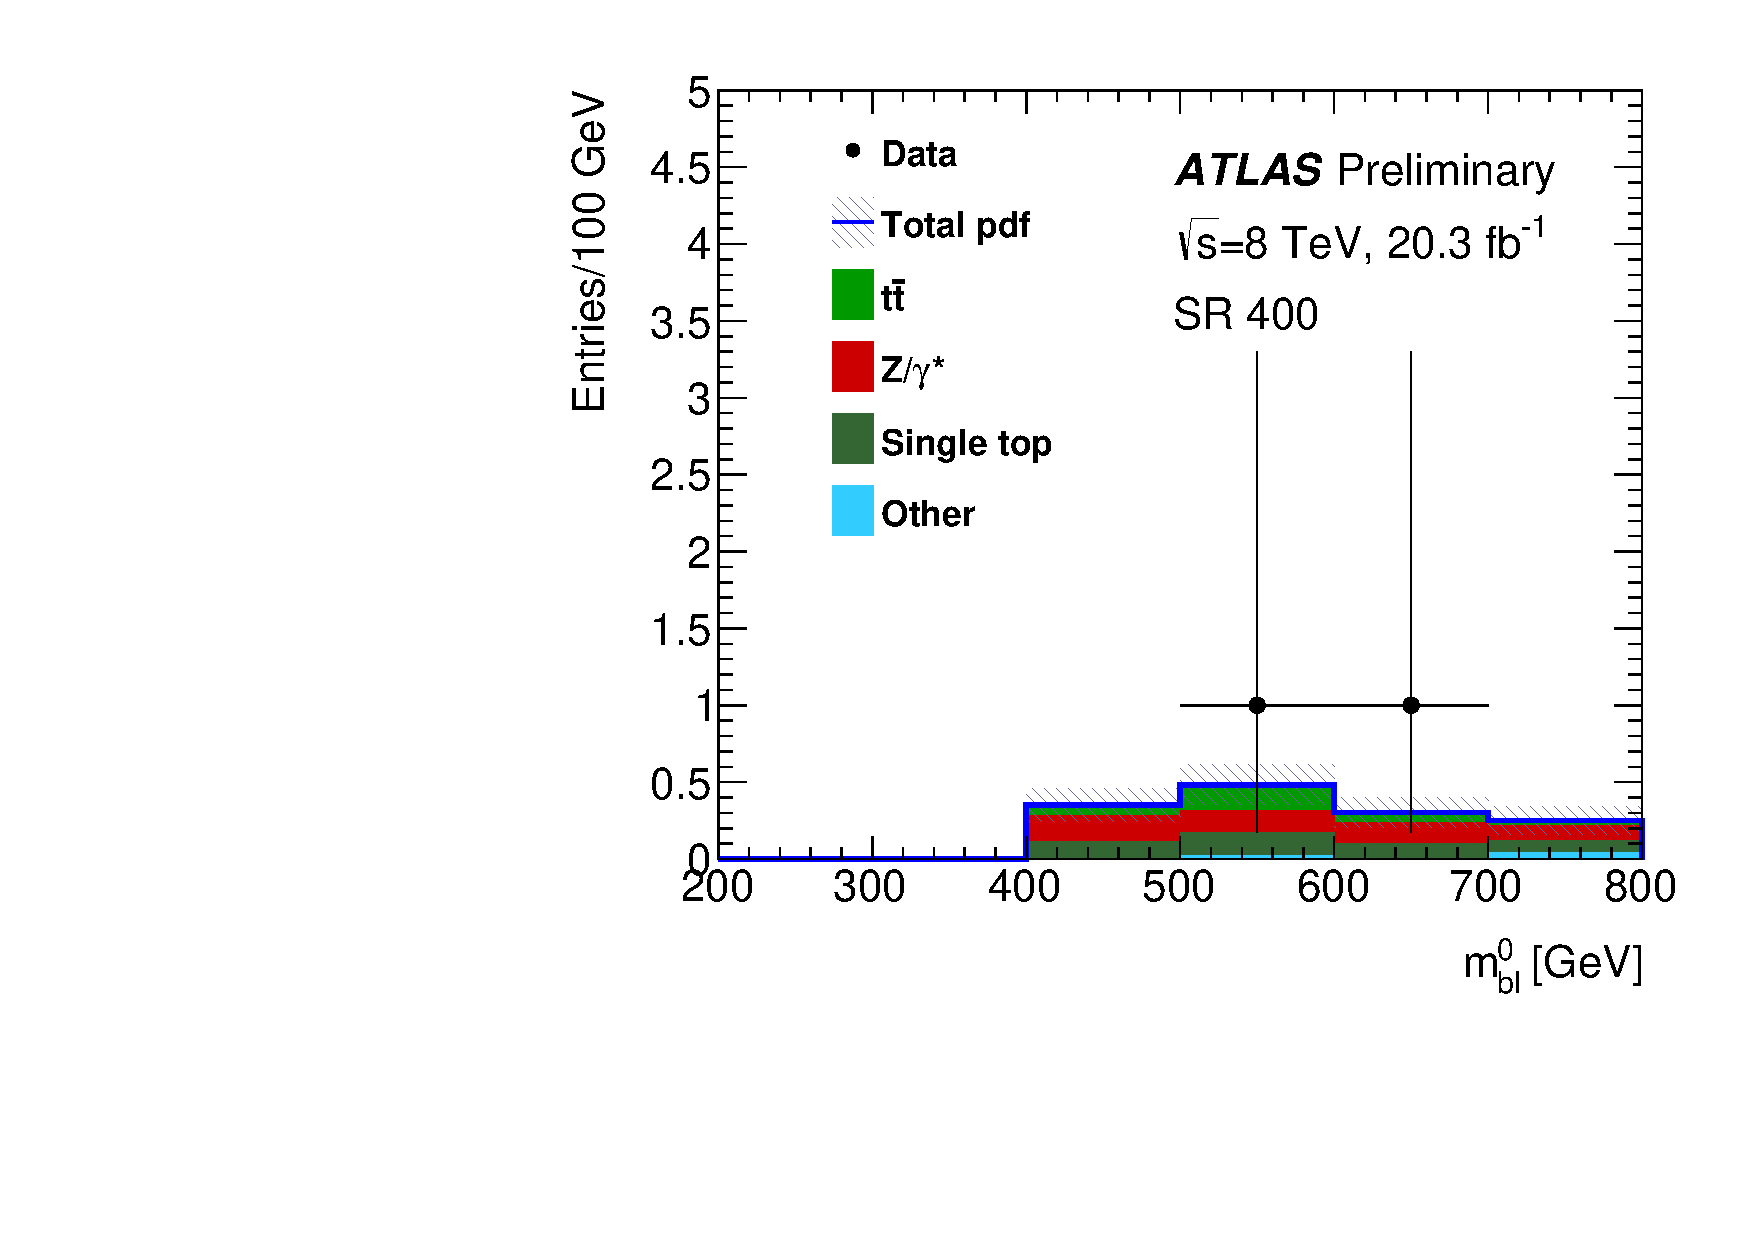
\includegraphics[width=0.45\textwidth]{figs/blstop/sr_mbl_0.pdf}
  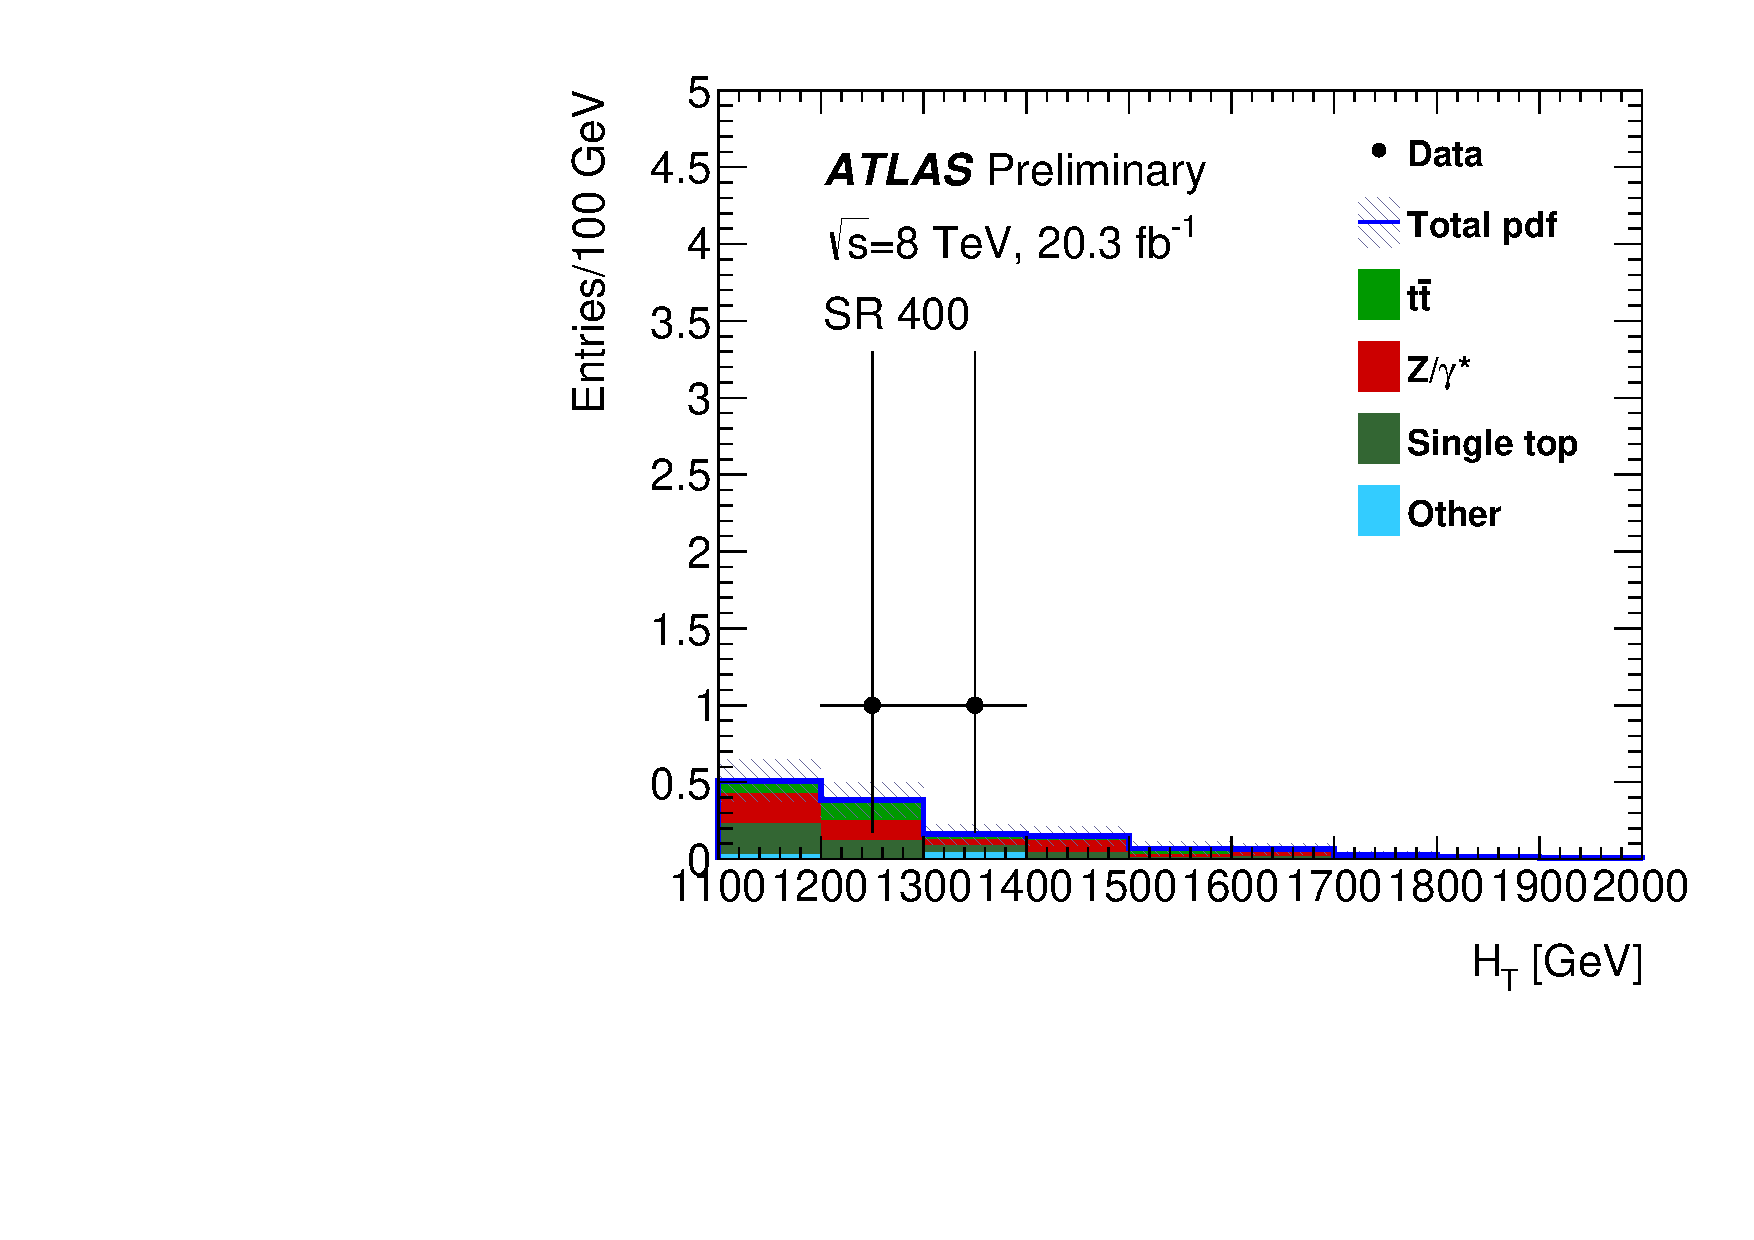
\includegraphics[width=0.45\textwidth]{figs/blstop/sr_ht.pdf}
  \caption{These plots show the $\MBL^0$ (left) and \HT\ (right) distributions
    in SR 400. The Standard Model background prediction is taken from the
    fitted background prediction. The hashed bands show
    the uncertainty on the fitted background prediction including the MC
    statistical and sources of systematic uncertainty.  The bottom of
    each plot shows the ratio of the observed data to the Standard Model
    background prediction.
  }
  \label{fig:sr_dists}
\end{figure}

As the observed number of events is consistent with the Standard Model
prediction, Upper limits at 95\% confidence level (CL) on the number of
beyond the Standard Model (BSM) events for each signal region are derived
using the $CL_s$ prescription and neglecting any possible contamination in the
control regions. Normalizing these by the integrated luminosity of the data
sample they can be interpreted as upper limits on the visible BSM
cross section, $\sigma_\mathrm{vis}$, where $\sigma_\mathrm{vis}$ is defined
as the product of acceptance, reconstruction efficiency and production
cross section. The results are given in
Tables~\ref{tab:event_yields_sr_400}~and~\ref{tab:event_yields_sr_600}.

Exclusion limits on the signal model are determined using the $CL_S$
prescription based on a simultaneous fit of the SRs and
CRs~\cite{Baak:2014wma}. The predicted signal contamination is
taken into account in the CRs.  For each stop mass,
exclusion fits are performed with various assumptions on the branching
ratios of the stop. For each point on the branching ratio plane, the
SR which provided the best expected sensitivity, as
measured by the lowest expected $CL_S$ value, is chosen. The expected
and observed limits are shown in Figure \ref{fig:limit_contours}. This figure
shows, for each simulated stop mass, the observed (expected) 95\% exclusion
limit on the 
branching fraction under the red (blue) line. A yellow band shows the
$\pm 1\sigma$ uncertainty on the expected limit, determined from the
systematic uncertainty on the signal and background prediction excluding
the effect of the signal cross section uncertainty.  The effect of varying
the signal cross section on the observed limit is indicated by the dashed
red lines.  The final limit on the stop mass is shown in
Figure~\ref{fig:mass_limit_obs}.  This plot shows the 95\% confidence
limit~(CL)
on the mass obtained by choosing the maximum excluded mass for each
branching ratio on the plane using the nominal cross section value.  
As the branching ratio of $\tilde{t} \rightarrow b\tau$ increases, the number
of expected events with electrons or muons in the final state decreases
for the same simulated stop mass. Therefore, the limit on the mass is
strongest at the bottom of the plane. In the top corner of the plot, the
SRs described in this analysis note have no sensitivity, however traditional
lepto-quark searches for final states with $b$-tagged jets and $\tau$ leptons
are able to place experimental limits in this region \cite{ATLAS:2013oea}.

\begin{figure}[ht]
  \centering
  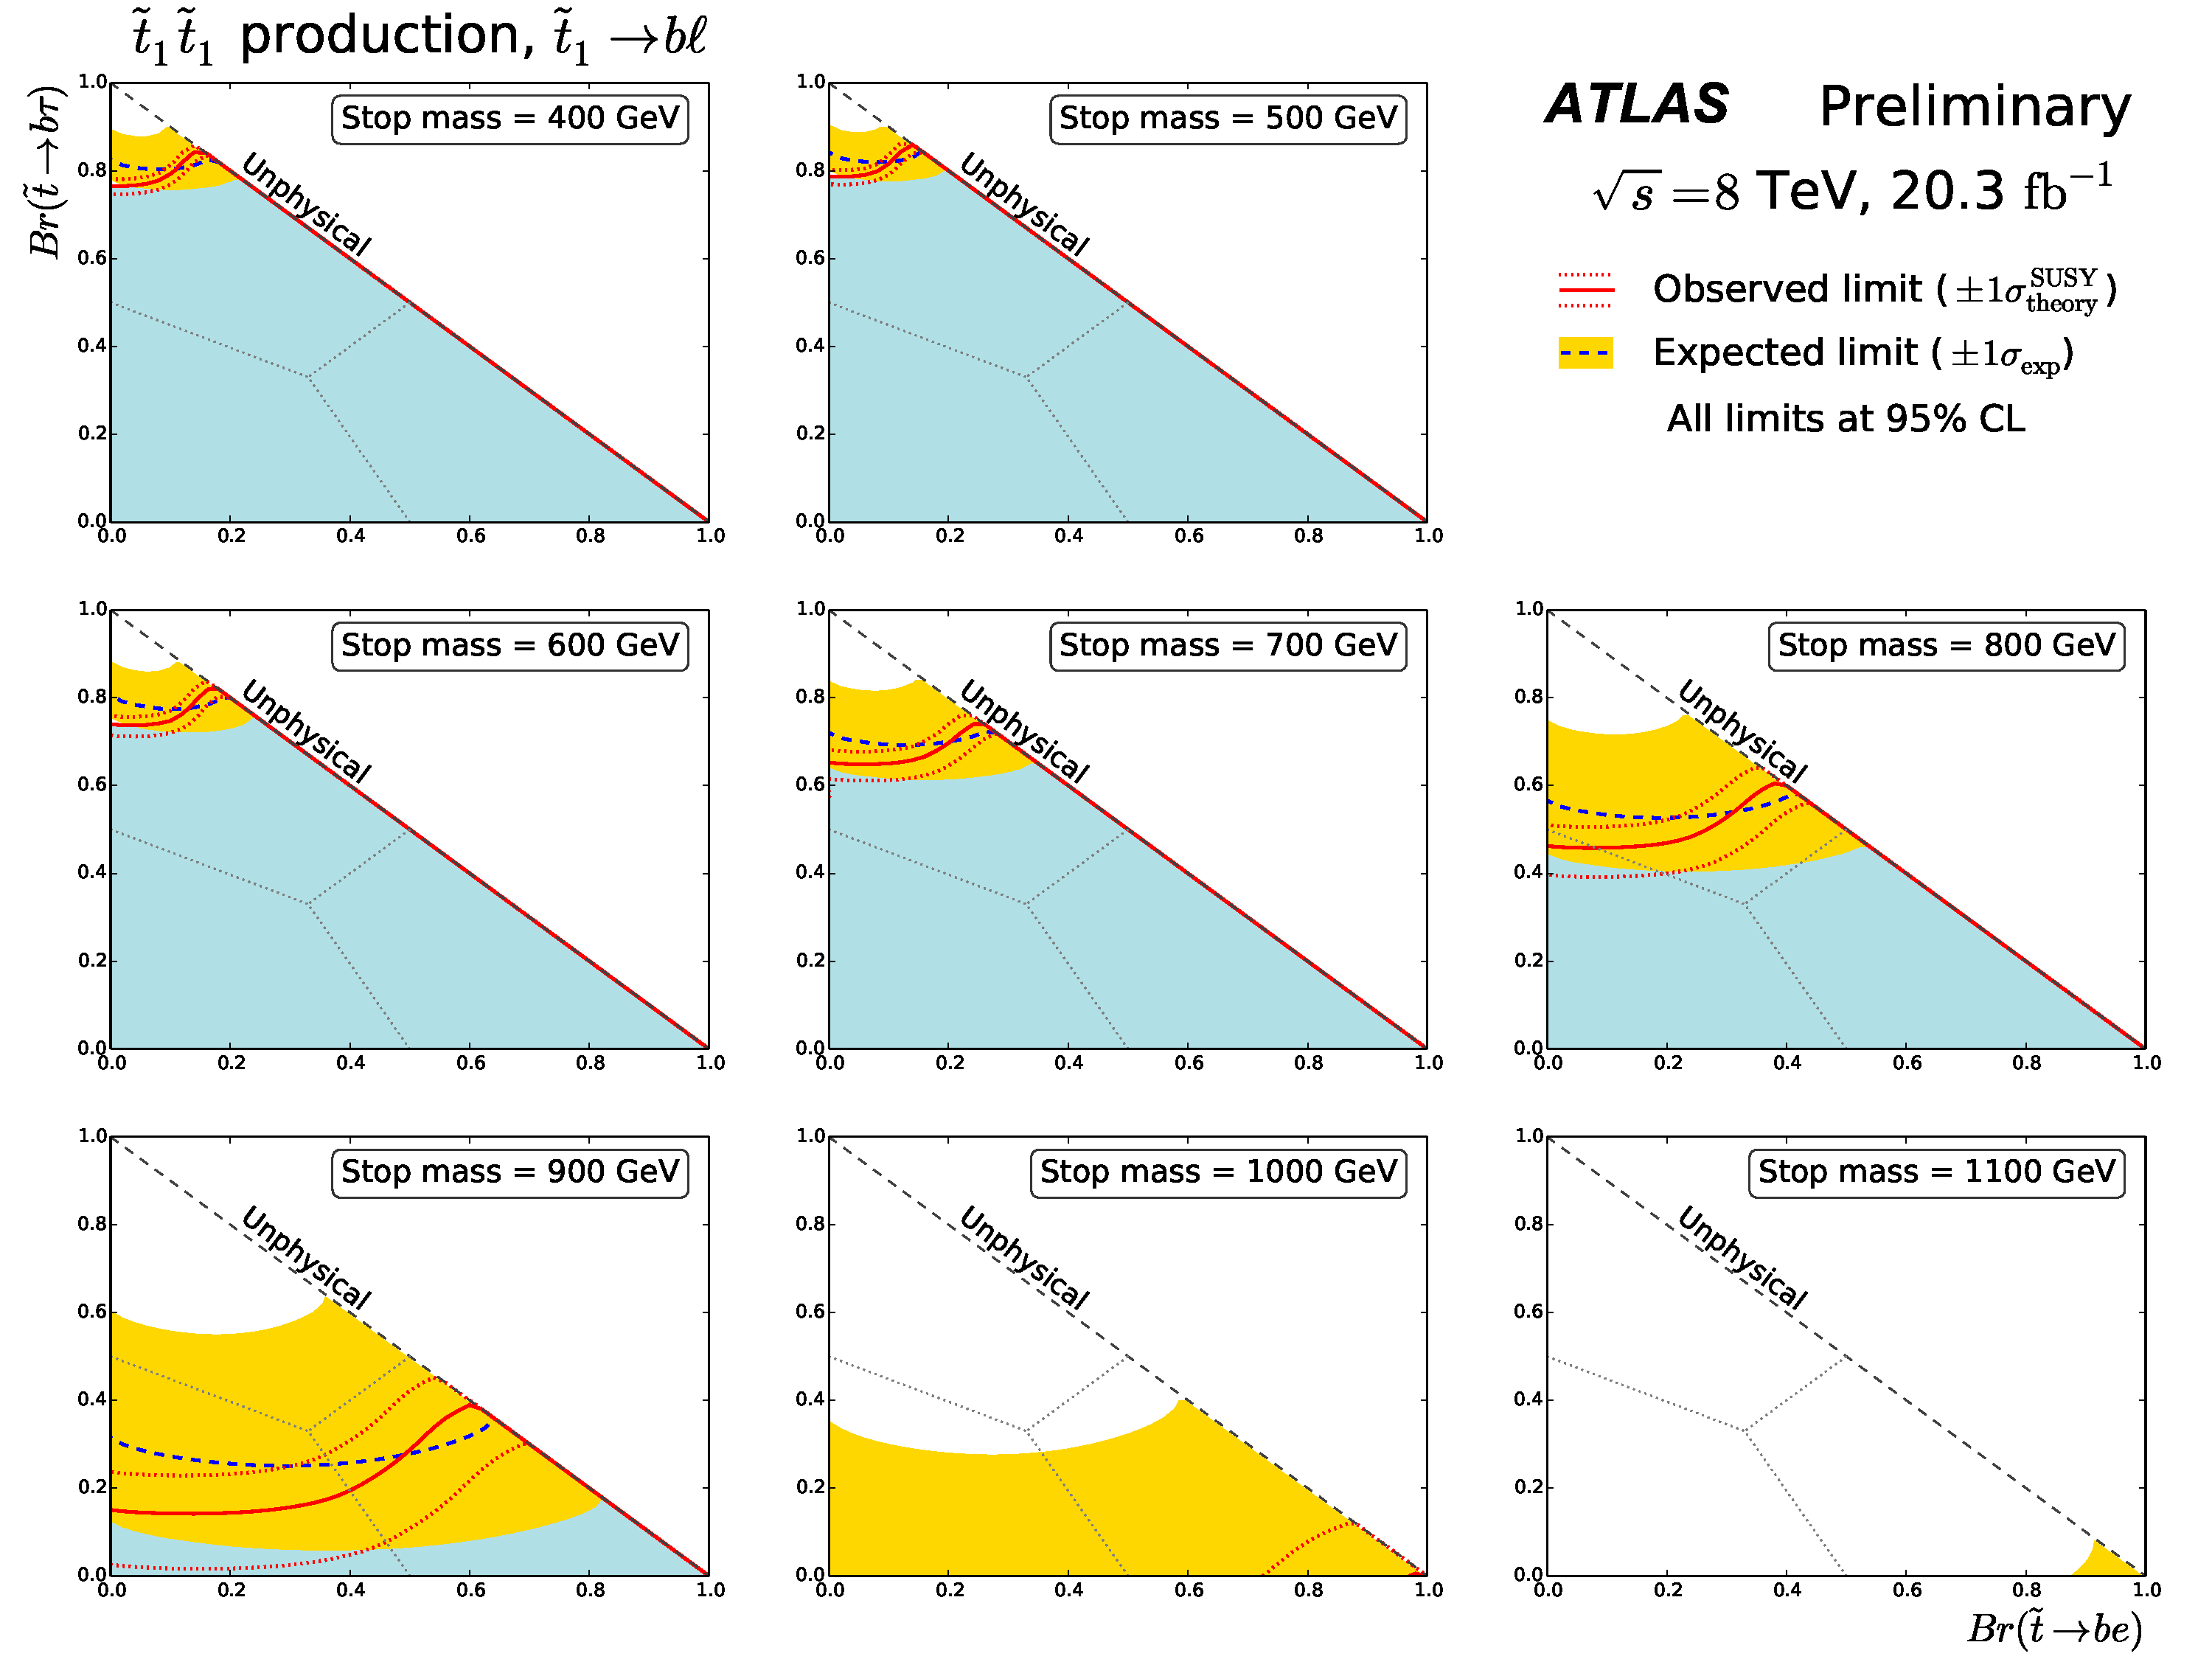
\includegraphics[width=\textwidth]{figs/blstop/limit_contours.pdf}
  \caption{Expected and observed limit on the branching ratios for the stop
    decaying to different lepton flavors shown for different stop mass
    hypotheses between 400 GeV and 1 TeV. The shaded area under the solid
    line represents the branching ratios which are excluded at 95\% CL
    for each stop mass.
    The dotted lines represent the uncertainty on the observed mass limit
    obtained by varying the signal model cross section up and down one standard
    deviation from the nominal value. The dashed line shows the
    expected 95\% CL exclusion for each stop mass, and the shaded band shows
    the uncertainty on this expected exclusion limit from statistical
    uncertainty and the sources of systematic uncertainty discussed in
    Section~\ref{sec:systematics}.
  }
  \label{fig:limit_contours}
\end{figure}

\begin{figure}[ht]
  \centering
  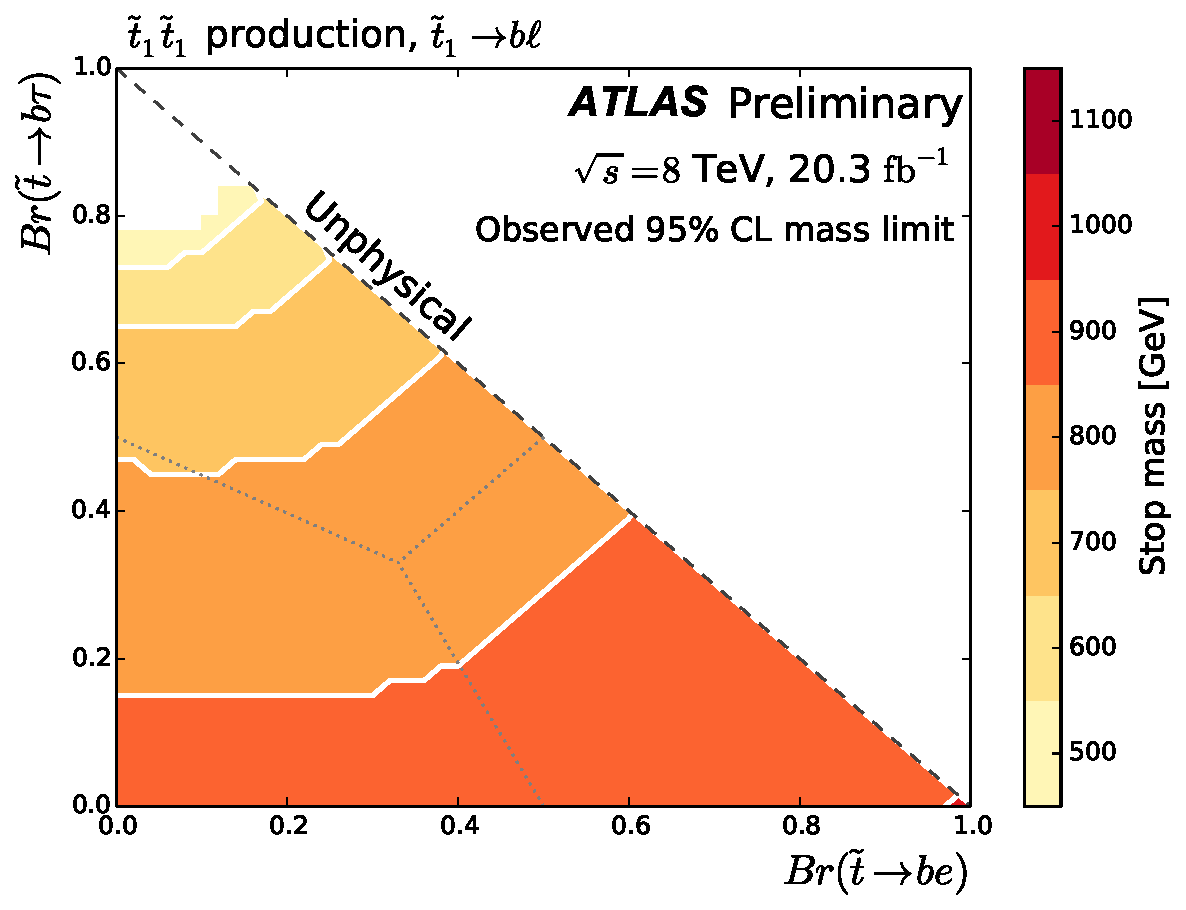
\includegraphics[width=0.6\textwidth]{figs/blstop/mass_limit_contours_no_extras_obs.pdf}
  \caption{The observed mass limit on the stop at 95\% CL.
    This limit is obtained using the nominal stop cross section.
    Stop masses between 400 \GeV\ and 1100 \GeV, in steps of 100 \GeV, were
    tested. The mass limit shown corresponds to the highest-mass stop sample
    which was excluded.
    As the branching ratio of $\tilde{t} \rightarrow b\tau$ increases, the
    number of expected events with electrons or muons in the final state
    decreases. Therefore, the limit on the mass decreases.
  }
  \label{fig:mass_limit_obs}
\end{figure}

%% -----------------------------------------------------------------------------
\section{Proposed improvements}
\label{sec:improvements}

